\documentclass[onecolumn, draftclsnofoot,10pt, compsoc]{IEEEtran}
\usepackage{graphicx}
\usepackage{url}
\usepackage{setspace}
\usepackage{caption}
\usepackage{longtable}

\usepackage{enumitem}
\setlist[itemize]{noitemsep, topsep=0pt}

\usepackage{titlesec}
\titleformat{\paragraph}[hang]{\normalfont\fontfamily{phv}\fontsize{9}{14}\itshape}{\theparagraph}{1em}{}
\titlespacing{\paragraph}{0pt}{1em}{0em}

\titleformat{\subparagraph}[hang]{\normalfont\fontfamily{phv}\fontsize{8}{12}\bfseries}{\theparagraph}{1em}{}
\titlespacing{\subparagraph}{10pt}{1em}{0em}

\usepackage{geometry}
\geometry{textheight=9.5in, textwidth=7in}

% 1. Fill in these details
\def \CapstoneTeamName{		    Nitro ChatBot}
\def \CapstoneTeamNumber{		63}
\def \GroupMemberOne{			Jack Barnes}
\def \GroupMemberTwo{			Sarun Pitaksuteephong}
\def \GroupMemberThree{			Cheng Xie}
\def \CapstoneProjectName{		ChatBot for Load Balancer Infrastructure}
\def \CapstoneSponsorCompany{	OSU Information Services}
\def \CapstoneSponsorPerson{	Stacy Brock}

% 2. Uncomment the appropriate line below so that the document type works
\def \DocType{	%Problem Statement
				%Requirements Document
				%Technology Review
				%Design Document
				%Progress Report
				Final Report
				}

%%%%%%%%%%%%%%%%%%%%%%%%%%%%%%%%%%%%%%%
\begin{document}
\begin{titlepage}
    \pagenumbering{gobble}
    \begin{singlespace}
        \hfill
        \par\vspace{.2in}
        \centering
        \scshape{
            \huge CS Capstone \DocType \par
            {\large\today}\par
            \vspace{.5in}
            \textbf{\Huge\CapstoneProjectName}\par
            \vfill
            {\large Prepared for}\par
            \Huge \CapstoneSponsorCompany\par
            \vspace{5pt}
            {\large Prepared by }\par
            Group\CapstoneTeamNumber\par
            \CapstoneTeamName\par 
            \vspace{5pt}
            {\Large
                \GroupMemberOne\par
                \GroupMemberTwo\par
                \GroupMemberThree\par
            }
            \vspace{20pt}
        }
        \begin{abstract}
            This document details the progress in design and development of CS63's Capstone project, Nitro Chatbot, for the school year ending June 2020.
            Nitro Chatbot is a chatbot interface that allows users to quickly access the status us, and modify basic configurations for their load balanced resources on a Citrix NetScaler.
            This report contains documentation developed by the team, the agreed-upon requirements of the project, and the state of the project as it hits version 1.0.
        \end{abstract}     
    \end{singlespace}
\end{titlepage}
\newpage
\pagenumbering{arabic}
\setcounter{tocdepth}{4}
\tableofcontents
\listoffigures
\listoftables
\clearpage


\section{Foreword}
\subsection{Release Notes 1.0}

This Final Report details the design and development Nitro Chatbot up to it's version 1.0.
Nitro Chatbot was developed from the proposed project idea "Chatbot for Load Balancer Infrastructure".
In it's current state, the project is fully functional, with it's stack able to fully launch in AWS from template.
Further development on Nitro Chatbot would likely be aimed towards adding new commands for a user to use.
These commands could include adding and removing resources, adding or removing bindings, and updating offloaded certificates.
Another change could be to modify the fields returned by status commands.
Details about potential further work to do on this project are contained in Appendix 2
All in all, we are satisfied with our progress on this project and hope that you are too.

\section{Introduction}
Nitro Chatbot began as the project proposal "ChatBot for Load Balancer Infrastructure", original proposed by Stacy Brock working at Oregon State University (OSU) in Information Services.

At OSU, load balancing is provided as a service to departments across campus.
Load balancing is the process of distributing network traffic across multiple servers, allowing for scaleable pools of redundant servers.
This process improves server responsiveness, and availability.
Users who manage these load balanced resources need to be able to view the status of, or modify configurations for them.
This may be in times of maintenance, or if a problem is detected elsewhere.
The problem is that these common tasks are cumbersome to access and execute, or may require attention from other employees to complete.

Nitro Chatbot aims to alleviate these issues by providing a mechanism to quickly access these common tasks from anywhere.
Nitro Chatbot provides an easy to use interface through Microsoft Teams that leverages built-in authentication to allow users to perform these common tasks.

Our team is composed of 3 members:
\begin{enumerate}
    \item Cheng Xie, who is responsible for the Chatbot component.
    \item Jack Barnes, who is responsible for the Relay component.
    \item Sarun Pitaksuteephong, who is responsible for the Deployment component.
\end{enumerate}

Our client, Stacy Brock, as a software engineer herself, provided a huge amount of support through the design phase and beyond.
Her expertise, knowledge of technologies, and methods were instrumental in assisting this project to fruition.

For anyone who wishes to continue to develop this project, I will refer you to Appendix 4, which contains any remaining work that may need to be done on this project.

\section{Requirements Document}
\subsection{Abstract}
This document is an SRS (Software Requirement Specification) which outlines the client requirements for the proposed chatbot software.
The chatbot will enable users to directly query the status, and modify configurations, for their load balanced resources.
The requirements within this document serve as a contract with the client and will be used to judge the quality and completeness of the software upon it's 1.0 release.

\subsection {Change History}
\begin{longtable}{ | p{1in} p{1in} p{4in} | }
 \caption{Requirements Document Change History}
 \\\hline
 \textbf{Revision} & \textbf{Date} & \textbf{Changes} \\
 \hline
 1.0 & 10/26/2019 
 & First Draft \\
 \hline
 1.1 & 11/25/2019 
   & - Added language to require direct messages for user commands \\
 & & - Modified language to allow for an additional authentication step. Added mention of a 60 second command response time limit.\\
 \hline
 1.2 & 12/03/2019
   & - Fixed broken symbol.\\
 & & - Correct spelling error.\\
 & & - Created table for user commands.\\
 & & - Updated both figures.\\
 \hline
 1.3 & 04/27/2020
 &   - 1.3.2 Removed first product function (Chatbot has it's own app window and does not need to listen for it's name).\\
 & & - Removed references to pools (replaced with generalized term: resources).\\
 & & - Removed requirement for updating certificates.\\
 & & - Removed usage of the university's federated login system, instead built-in authentication in Microsoft Teams is used. \\
 & & - Removed reference to stateless functionality, which does not work for this type of application. \\
 \hline
 1.3.1 & 04/27/2020
   & - 2.1 Testing suites target input checking (as the application does not easily allow for live testing with it's web services implementing additional built-in security to safeguard traffic).\\
 & & - 2.2 Removed reference to additional persistent storage (this requirement is unneeded).\\
 & & - 2.3 Updated Table 1 (Available user commands). Added: list, listall, listbound, disablenow, help, request-auth, Removed: updatecert.\\
 & & - 2.5 Removed reference to additional authentication step (This is unneeded for the used authentication pattern).\\
 & & - Changed reference to "remove" command to "disable".\\
 & & - Removed "Logical database requirements" section (formerly 2.7), as no database is needed.\\
 \hline
 2.0 & 05/25/2020
   & - Updated overview figure and gantt timeline figure.\\
 \hline
\end{longtable}

\subsection{Introduction}
\subsubsection{Purpose}
 The software will provide a chatbot interface for users to query the status of their load balanced resources within the Oregon State University network.
 Users with the correct permissions will be able to quickly access the status and perform common configuration tasks on the University's load balancer.
 
\subsubsection{Scope}
Two primary software components will need to be developed.
The first is the chatbot that will accept commands from a user.
The second software will act as the internal relay, receiving requests from the chatbot, sending commands to the load balancer and then returning the results.
The relay will maintain authentication for active users and perform the direct interaction with the load balancer API (Application Program Interface).
This will allow the chatbot to provide quick access to the status and configuration options for the server pools that the users manage.

\subsubsection{Product overview}

\paragraph{Product perspective}
Chatbots are typically used in dialog systems for various practical purposes including customer service or information acquisition \cite{chatbot}.
This proposed implementation of the chatbot exists on top of an existing system and is meant to provide convenient access for the target users.
The chatbot itself will operate as the user interface for users to direct message.
The internal relay will operate as a software interface with the Citrix NetScaler, using it's REST API \cite{citrixnitro}.

\paragraph{Product functions}
The software will have the following major functions:
\\1. The chatbot will accept input from the user and parse input for commands.
\\2. Upon parsing a command, it will securely transmit command and user information to the internal relay.
\\3. The relay will manage authentication
\\4. The relay will send requests to the load balancer through NITRO API
\\5. The relay will transmit results back to the chatbot.
\\6. The chatbot will respond appropriately to user commands.
\\7. The user will not have to authenticate separately outside of Microsoft Teams.
\\8. Users will be able to query for the status resources (including vservers, servicegroups, services, and servers).
\\9. Users will be able to query for the status of individual servers.

\paragraph{User characteristics}
Users of this chatbot will be system administrators who manage pools of servers at Oregon State University. They have ONID (OSU Network ID) accounts. They have a high-level of technical understanding and are familiar with command line interfaces. The targeted user base is approximately 2 dozen people.
\paragraph{Limitations}
The chatbot will operate on a common platform accessible to all targeted users.
It will leverage the built-in authentication within Microsoft Teams to identify users.
The chatbot must be written in a framework that ensures future portability.
The chatbot itself must be stateless, and not requiring persistent storage.
The chatbot should be (virtually) always available, running on a cloud service within public internet.
A system of CI/CD (Continuous Integration / Continuous Deployment) must also be developed to maintain availability.

\subsubsection{Definitions}
\underline{Botkit Framework}: An open-source developer tool for building chatbot that also allows custom integration for major messaging platforms. Has direct access to platform APIs. It is owned by Microsoft \cite{framework}.
\\\underline{Chatbot}: A chatbot is a piece of software that conducts a conversation via auditory or textual methods \cite{chatbot}.
\\\underline{Citrix NetScaler}: A an application delivery controller made by Citrix that load balances to make sure that applications can be run as smooth as possible \cite{netscaler}.
\\\underline{Duo}: It is a vendor for cloud-based two-factor authentication service. It can be integrated with any website, VPN (Virtual Private Network), and cloud services \cite{duo}.
\\\underline{Load Balancer}: Load balancer is a reverse proxy that distributes network or application traffic across the server pool. This will increase the efficiency, maintainability, and, speed of the server pool. 
\\\underline{NITRO API}: The NetScaler NITRO protocol allows you to configure and monitor the NetScaler appliance programmatically by using Representational State Transfer (REST) interfaces \cite{citrixnitro}.
\\\underline{ONID}: Oregon State University ID used for identification
\\\underline{REST}: Representational State Transfer. It is a software architect style that defines what could be used for creating web services. The main constraint are the client that uses the API and the resources that the API can provide information to \cite{restphd} \cite{rest}.

\subsection{Requirements}
\subsubsection{Apportioning of requirements}
Two separate pieces of software will be defined in these requirements.
This first is referred to as the chatbot, and the second piece of software is referred to as the relay.
These separate pieces of software will be developed separately, but concurrently.
Both have features that rely on the operation of the other.

To assist with development, tests will be written to check input and parsing of that input.
Features and requirements that span both the chatbot and the relay may be implemented in this fashion at first.
However the feature will not be considered fully implemented until both component software operate with each other.

\subsubsection{Specified requirements}
The first component software is the chatbot.
The chatbot will run from from a cloud service and operate within a chat platform that can be equally accessed by all users.
The chatbot will be triggered to begin processing input when it's messaged directly, and will not operate by idling within a channel and parsing messages.

When a user messages the chatbot, it will begin parsing input given to it in a manner consistent with command line interfaces.
If the input is invalid, it will tell the user.
If the input in valid, it will initiate communication with the second component software, the relay.
The chatbot will send a request to the relay containing all the necessary information to complete the request, including user information.

When the relay receives a request, it will use the user information to request authentication from the NetScaler.
The relay will communicate requests to the NetScaler using it's REST API, NITRO API.
The relay will maintain and manage authentication in a manner that meets the software requirements.

After a user is authenticated, the relay will send the command request to the NetScaler.
Upon receiving a reply from the NetScaler, the relay will format a reply and send it to chatbot.
The chatbot will then format and send the result to the user.
    
\subsubsection{Functions}
The perspective of the user, the functioning of the software will be quiet simple, with only a small number of commands available.
The intention of the software is to perform these complex configuration tasks as seamlessly as possible.
The chatbot will parse commands from a user when a user directly messages it.
The available functions are detailed below:
\begin{longtable}[h]{ | p{1.85in} | p{2.7in} | p{1.95in} |  }
     \caption{Available User Commands}
     \\\hline
     \textbf{Command} & \textbf{Description} & \textbf{Response} \\
     \hline
     list
     & List all vservers
     & Returns a list of all vservers\\
     \hline
     listall
     & List all resources
     & Returns a list of all resources\\
     \hline
     listbound $<$resource$>$
     & Lists all resources bound to the specified resource
     & Returns a list of resources, or an error if it's a server \\
     \hline
     status $<$resource$>$
     & Query the status of a resource
     & Returns a list of resource properties, including it's state \\
     \hline
     enable $<$resource$>$
     & Enable the server within it's pool
     & Confirmation of success \\
     \hline
     disable $<$resource$>$ [delay]
     & Disables a resource gently, with an optional delay
     & Confirmation of success \\
     \hline
     disablenow $<$resource$>$ [delay]
     & Disables a resource (not gently), with an optional delay
     & Confirmation of success \\
     \hline
     help [command]
     & Displays a usage text, or optionally, for one command
     & Returns all usage text, or a single usage text \\
     \hline
     request-auth [message]
     & Sends a request to the admin for access (message is optional)
     & Confirmation that the log was sent \\
     \hline
\end{longtable}

If a user asks to perform a task without proper having permissions, then the bot will respond to the user that they do not have permission to perform the requested task.

\subsubsection{Performance requirements}
The chatbot is to be, essentially, always available.
It is expected to run continuously on a cloud server, responding to a user when it's messaged directly.
Each user command should be received, processed, and be responded to in a manner of seconds (with 60 seconds being an upper limit).
The chatbot should process commands concurrently, never needing to finish previous requests before new requests are received.
The chatbot should be able to receive command input from multiple sources simultaneously without losing received requests ($<$1\% dropped input). 

\subsubsection{Usability requirements}
For the user, sending commands through the chatbot should be a seamless experience, minimizing the number of required steps to perform a task.
To achieve this, the chatbot must minimize user interaction while maintaining security.

The chatbot will accept commands from authorized users in a similar style to command line utilities.
The formatting of the interaction will be first the command, then any applicable flag, followed by additional information.
For example, a user may ask the bot to disable webserver2 by inputting: "disable webserver2".

\subsubsection{Interface requirements}
For proper operation and integration of the chatbot and it's relay, both have a number of existing systems that they must interface with.

The chatbot must be deployed to a cloud service to maintain availability. 
This includes designing a system of continuous integration/deployment to allow for remote deployment.
The chatbot must also interface with the chosen chat platform.
Finally, the chatbot must remotely interface with it's relay using a secure connection and common language, through which, it can communicate with the relay.

The relay, the second piece of software, will eventually be deployed internally within the Oregon State University network.
To achieve this, it will likely be deployed as a virtual machine, however the details of this deployment are not statically specified at this time.
However, for development, the relay will be deployed to a cloud instance.

The relay must accept a secure connection from the chatbot (which is deployed remotely).
The relay must interpret user information contained within requests from the chatbot to identify and authenticate against the load balancer (Citrix NetScaler).
The relay will interpret commands and send requests to the Citrix NetScaler using it's REST API, NITRO API.

\subsubsection{Design constraints}
The chatbot will be deployed to a cloud service in a manner that allows continuous deployment and continuous integration. 
The relay must utilize the Nitro API to communicate with the NetScaler. 
The chatbot must have a separate relay so that it does not communicate directly with the load balancer.

\subsubsection{Software system attributes}

\paragraph{Reliability}
The chatbot or the relay should not crash or produce unspecified states regardless of user input or data received from any interface. 
If the software does halt, or reach an unspecified state, it must be deployed it such a manner that it restarts and restores itself with minimal loss of data or downtime.

\paragraph{Availability}
The chatbot is intended to be always available.
One exception is the availability of the cloud server/service it's deployed to.
An additional factor in availability, will be the implementation of a messaging system between the chatbot and the relay.
This system must account for connection instability resulting from any number of factors.

\paragraph{Security}
Security is paramount with the implementation of this software system, as the chatbot will be indirectly communicating with vital network resources.
Users must never be able to request information about, or reconfigure, network resources they don't have explicit permission to modify.

All reconfiguration and status requests must be logged and made accessible to only administrative users.

The relay must interpret requests from the chatbot, never directly passing queries from the chatbot.
The relay must minimize the amount of information that is sent to the chatbot, relaying only what is necessary.

Additionally, the chatbot must never monitor messages that aren't directed at it.

\paragraph{Portability}
In an attempt to future-proof the chatbot, it will be written using a portable framework.
This will allow the chatbot to be easily portable to different messaging networks, minimizing the work required if an organizational transition occurs.


\section{Design Document}
\subsection{Abstract}
This document outlines the entire design of the software project known as Nitro Chatbot, which is the proposed solution to the project proposal "ChatBot for Load Balancer Infrastructure".
This document serves as an informative document for the development team to communicate a detailed blueprint of the proposed design to the stakeholders.
Nitro Chatbot is comprised of 3 main components (Chatbot, Relay, Deployment) that work in unison to provide a solution.
The chatbot (deployed to AWS) will connect to Microsoft Teams, accept command input, authenticate users, forward requests to the relay, receive replies and display them to the user.
The relay will await requests from the chatbot, forward them to the load balancer, and return the response to the chatbot.
Finally, the deployment module describes the continuous integration/continuous deployment (CI/CD) pipeline used to rapid and reliable development.

\subsection {Change History}
\begin{longtable}{ | p{1in} p{1in} p{4in} | }
 \caption{Design Document Change History}
 \\\hline
 \textbf{Revision} & \textbf{Date} & \textbf{Changes} \\
 \hline
 1.0 & 11/25/2019 
   & - First Draft\\
 \hline
 1.1 & 12/03/2019 
   & - Both figures have been updated to the latest versions.\\
 & & - Language has be clarified that users must use direct messages to send commands to the chatbot.\\
 & & - User commands have been consolidated into a table.\\
 & & - Deployment have been changed to an EC2 instance to meet the availability requirement.\\
 & & - Administrative specifications clarified. \\
 \hline
 2.0 & 05/25/2020 
   & - 1.4 Removed definition for Duo\\
 & & - Figure 1 Updated project overview image.\\
 & & - 2.1 Moved authentication to the backend (Relay). Removed reference to CDK, as the final solution was exclusively built as a CloudFormation template.\\
 & & - 2.2 Changed "mentioned" to "messaged".\\
 & & - 3.1.1 Removed authentication from the frontend. Added reference to HTTPS. Updated command table. Added mention of TOTP key.\\
 & & - 3.1.2 Removed mention of IDP, added mention of HTTPS.\\
 & & - 3.2.1 Added verification of user's identity. Updated command table. Mentioned the use of HTTPS.\\
 & & - 3.2.2 Added interaction with AWS SecretsManager for retrieving credentials NetScaler.\\
 & & - 3.2.3 Removed connection renegotiation, added use of HTTPS.\\
 & & - 3.3.1 Removed reference to CDK, and added mention of CloudFormation template. Testing focus modified to state primary focus on input validation. Added information about Jenkins instance on AWS.\\
 & & - 3.3.2 Remove interactions with chatbot and relay. Added interactions with GitHub for CI, and with AWS for deploying.\\
 & & - 4.1 Added updated Gantt chart reflecting the actual development timeline. \\
 \hline
\end{longtable}

% 8. now you write!
\subsection{Introduction}

\subsubsection{Purpose}
Nitro Chatbot will provide a chatbot interface for users to query the status of their load balanced resources within the Oregon State University network.
Users with the correct permissions will be able to quickly access the status and perform common configuration tasks on the University's load balancer, a Citrix NetScaler.

\subsubsection{Scope}
Two primary software components will need to be developed.
The first component is the chatbot that will accept commands from a user.
The first component is known as the chatbot, but may also be referenced as the front-end or the user interface (UI), as it provides both of these functions for the software system.
The second component software will act as a relay, receiving requests from the chatbot, sending commands to the load balancer from within the network and then returning the results to the chatbot.
The relay is also known as the back-end as it performs actions out of view of the user.
The relay will maintain authentication for active users and perform the direct interaction with the load balancer API (Application Program Interface).
This will allow the chatbot to provide quick access to the status and configuration options for the server pools that the user's manage.

\subsubsection{Intended Audience}
Users of this chatbot will be system administrators who manage server pools at Oregon State University. They have ONID (OSU Network ID) accounts.
They have a high-level of technical understanding and are familiar with command line interfaces.
The targeted user base is approximately 2 dozen people.

\subsubsection{Definitions}
\underline{Botkit Framework}: An open-source developer tool for building chatbot that also allows custom integration for major messaging platforms. Has direct access to platform APIs. It is owned by Microsoft \cite{framework}.
\\\underline{Chatbot}: A chatbot is a piece of software that conducts a conversation via auditory or textual methods \cite{chatbot}.
\\\underline{Citrix NetScaler}: A an application delivery controller made by Citrix that load balances to make sure that applications can be run as smooth as possible \cite{netscaler}.
\\\underline{Load Balancer}: Load balancer is a reverse proxy that distributes network or application traffic across the server pool. This will increase the efficiency, maintainability, and, speed of the server pool. 
\\\underline{NITRO API}: The NetScaler NITRO protocol allows you to configure and monitor the NetScaler appliance programmatically by using Representational State Transfer (REST) interfaces \cite{citrixnitro}.
\\\underline{ONID}: Oregon State University ID used for identification
\\\underline{REST}: Representational State Transfer. It is a software architect style that defines what could be used for creating web services. The main constraint are the client that uses the API and the resources that the API can provide information to \cite{restphd} \cite{rest}.  
\\\underline{Server Pool}: An autonomous region that contains physical servers. It is a simplified unified view where virtual machines are located \cite{pools}.

\subsection{System Overview}
\begin{figure}[h]
    \centering
    \captionsetup{format=hang,justification=raggedright,margin=2cm}
    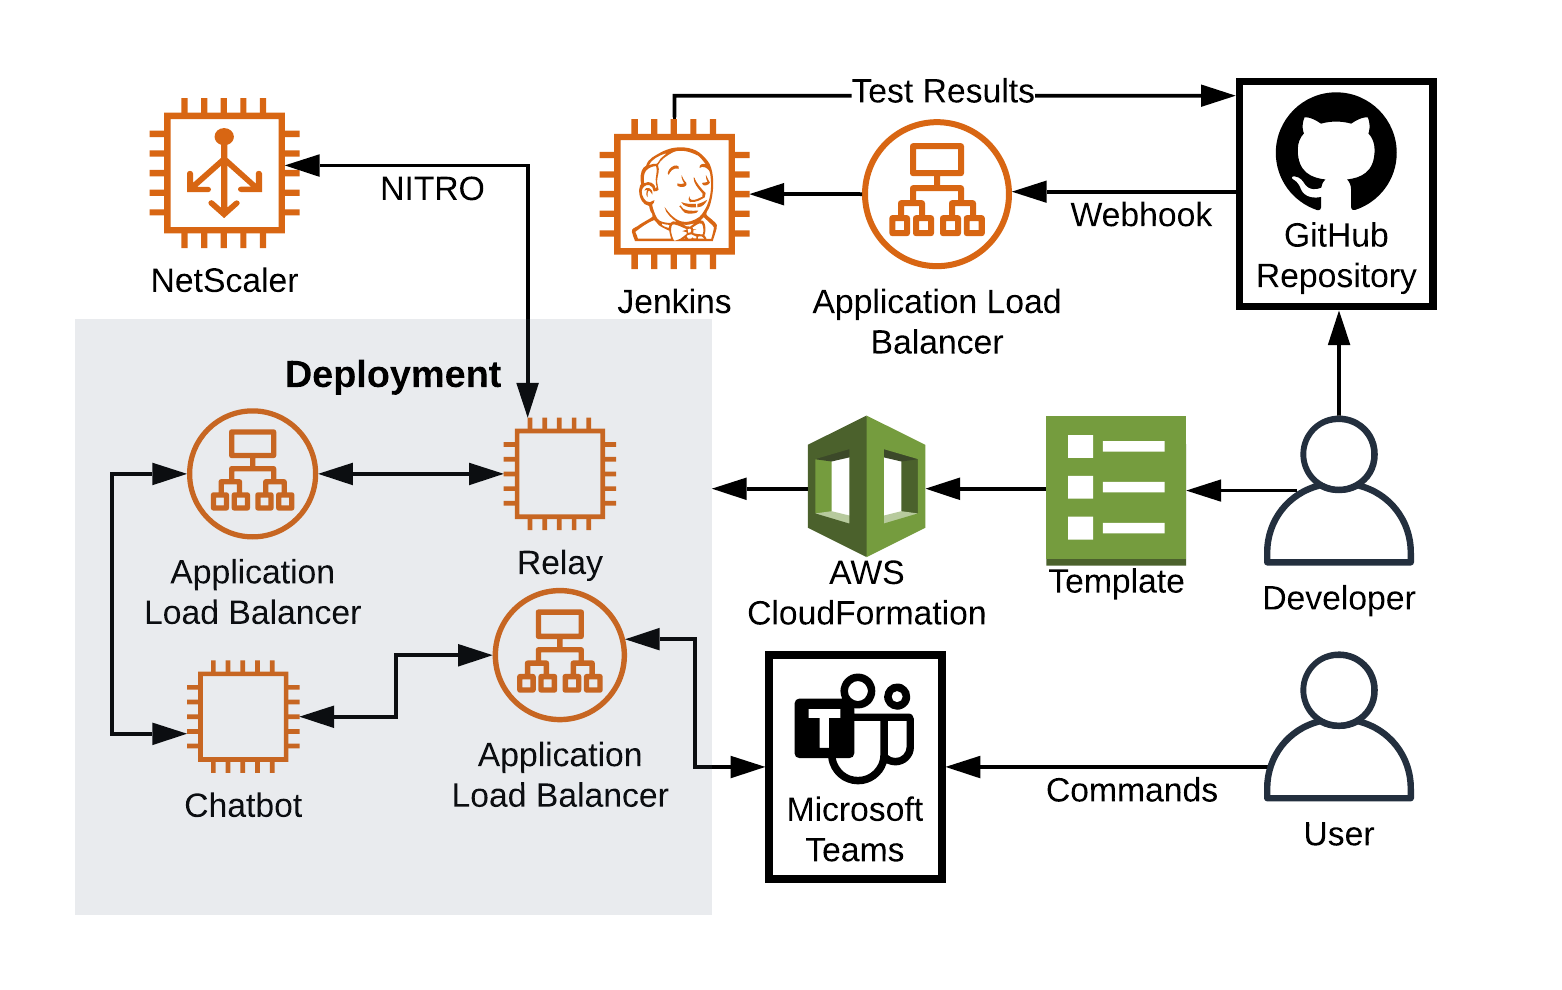
\includegraphics[height=9cm]{overview-v3.png}
    \caption[Basic overview of the chatbot]{Basic overview of the chatbot, and how it will allow users access to load balancer configurations.}
    \label{fig:Nitro Chatbot}
\end{figure}
\subsubsection{System Design}
Nitro Chatbot is comprised of 3 main components (chatbot, relay, deployment) that work in unison.

The first component, chatbot, is a piece of software written in Node.js.
It serves as the User Interface (UI) and as the frontend.
It will connect to Microsoft Teams, receive commands from the user, forward requests to the relay, and display responses from the relay.

The second component, relay, is a piece of software that is written in Node.js.
The relay serves as the backend of the software system.
It receives requests from the chatbot, verifies the identity of the user, formats and forwards them to the Citrix NetScaler (a load balancer). 
When it receives the response from the load balancer it formats the response and sends it to the chatbot.

The third component, deployment, describes the Continuous Integration / Continuous Deployment(CI/CD) pipeline that will be created to test builds and to deploy them into the production environment.
Jenkins will be used to run test suites that will be developed for both the chatbot and the relay.
Amazon Web Services CloudFormation will be used to deploy the software into production.

\subsubsection{Design Stakeholders and their Concerns}
Since Nitro Chatbot is designed to eventually integrate into existing infrastructure, stakeholder requirements are paramount to the successful development of this software system.
The chatbot component should be written using the Botkit framework, and it must be deployed to Amazon Web Services (AWS). 
It will receive commands from the user when messaged directly, not listening to messages at any other time.

The load balancer is a Citrix NetScaler running 12.0 software and will be communicated with using it's REST API: NITRO API.
The load balancer will be configured with partitions, so that each user can only configure their owned resources.
The chatbot must not directly communicate requests to Load Balancer, as this causes a security issue.

\subsection{Component Design}
\subsubsection{Chatbot}
\paragraph{Composition}
The first component of the Nitro Chatbot is a chatbot, which functions as the frontend (or user interface) for the software system.
The chatbot will be implemented in Node.js, utilizing available packages (libraries) to meet the requirements of the component.
At it’s core, the chatbot accepts commands from the user, input as messages directed at the chatbot.
If the command is a valid command, the chatbot will send the full details of the request to the relay.
When the chatbot receives a response from the relay, it will display it to the user.

To meet current stakeholder requirements, the chatbot will be designed to operate within Microsoft Teams, utilizing the Botkit Framework\cite{botkit}.

The first task for the chatbot is to establish a secure and encrypted connection with the relay.
A TLS (Transport Layer Security) connection will be implemented to connect the chatbot to the relay.
The chatbot will be responsible for initiating the connection to the relay via an HTTPS request.
The chatbot and the relay will communicate in the pattern of a reverse proxy, with the chatbot sending requests and expecting a response.

The primary task for the chatbot will be to wait for commands from users send direct messages to it.
When it detects a command from a user, it will attempt to parse it.
If it is a valid command, the chatbot will have the user authenticate.
Once authenticated, the chatbot will package the request as a JSON file and send it to the relay.
When the relay responds, the chatbot will format a response for the user and send it to them.
The chatbot will log all user interactions in Amazon Web Service (AWS) CloudWatch, removing sensitive information prior to storage.

\begin{longtable}[h]{ | p{1.85in} | p{2.7in} | p{1.95in} |  }
     \caption{Available User Commands}
     \\\hline
     \textbf{Command} & \textbf{Description} & \textbf{Response} \\
     \hline
     list
     & List all vservers
     & Returns a list of all vservers\\
     \hline
     listall
     & List all resources
     & Returns a list of all resources\\
     \hline
     listbound $<$resource$>$
     & Lists all resources bound to the specified resource
     & Returns a list of resources, or an error if it's a server \\
     \hline
     status $<$resource$>$
     & Query the status of a resource
     & Returns a list of resource properties, including it's state \\
     \hline
     enable $<$resource$>$
     & Enable the server within it's pool
     & Confirmation of success \\
     \hline
     disable $<$resource$>$ [delay]
     & Disables a resource gently, with an optional delay
     & Confirmation of success \\
     \hline
     disablenow $<$resource$>$ [delay]
     & Disables a resource (not gently), with an optional delay
     & Confirmation of success \\
     \hline
     help [command]
     & Displays a usage text, or optionally, for one command
     & Returns all usage text, or a single usage text \\
     \hline
     request-auth [message]
     & Sends a request to the admin for access (message is optional)
     & Confirmation that the log was sent \\
     \hline
\end{longtable}

If the user gives an invalid command, the chatbot will tell the user to try again.
If the user gives a valid command, then the chatbot will send the request to the relay.

With each request send to the Relay, a unique TOTP token (generated from a symmetric key and the current time), will be sent.
This will allow the relay to authenticate the source of the request. The symmetric key will be generated and distributed during deployment only.

The request will be packaged in a JSON, along with user information and the TOTP token, and then sent to the relay via HTTPS.
When a response is received from the relay, the chatbot will log the interaction and display the results to the user via Microsoft Teams.

Finally, the chatbot will utilize Jasmine for unit tests. This will allow Jenkins continuous integration (CI) to run the tests in an automated fashion.

\paragraph{Interactions}
The chatbot has many interactions that it must manage: users (via Microsoft Teams), the relay, and CloudWatch.

The chatbot acts as the user interface (UI) for Nitro Chatbot.
All user interactions are directly with the chatbot through Microsoft Teams.
The chatbot will only read messages that are sent directly to it.

The chatbot also interacts with the relay, through a Transport Layer Security (TLS connection) with HTTPS.

Finally, the chatbot must also log all user interactions.
The chatbot will utilize Amazon's CloudWatch to store logs that can be accessed at a later time.

\paragraph{Metrics and Additional Criteria}
The chatbot is responsible for establishing the TLS connection to the relay.

The chatbot must be able to receive multiple commands from multiple users simultaneously, and not lose/mishandle any requests.
Non-blocking behavior will require an asynchronous implementation.
Additionally, all requests must be responded to in a timely fashion.
Should any requests not receive a response, then the user should be notified of the error.
All requests are to be completed and responded to within 60 seconds.

The chatbot must be able to parse commands and determine their validity.
All information sent to the relay must be encrypted, as it contains critical credential information that could be misused if intercepted.

The chatbot is responsible for maintaining logs that can be reviewed by an administrator.
CloudWatchLogs includes an administrative panel that will allow for auditing by an administrator of the system.

\subsubsection{Relay}
\paragraph{Composition}
The second component of the Nitro Chatbot is a relay, which functions as the backend for the software system.
The relay will be implemented in Node.js, utilizing available packages (libraries) to meet the requirements of the component.
At it's core, the relay accepts requests from the chatbot (frontend), verifies the identity of the user, formats and forwards them to the load balancer (a Citrix NetScaler 12.0).
The load balancer replies to the relay, which in turn formats the response for the chatbot and sends it as a response to the request.
To achieve this program flow, several technologies and methodologies will be utilized.

A TLS (Transport Layer Security) connection will be implemented to connect the chatbot (which exists on public internet) to the relay (which may reside on a private network) via HTTPS.
The chatbot and the relay will implement a reverse proxy messaging pattern for communication.

The primary task for the relay is to wait for requests from the chatbot.
These requests will be formatted as JSONs, and contain all nessicary information to authenticate with the load balancer and complete the requested command.
It will fully process the request, sending it to the load balancer in the correct format.
When it receives a response from the load balancer, it will format and transmit a JSON response to the chatbot.

To communicate with the load balancer, the relay will utilize the available REST API: NITRO API \cite{nitro}.
The load balancer (Citrix NetScaler) will be running software version 12.0 and will have users and their owned resources configured into partitions.
This allows the relay to incorporate the the security principle of least privilege, which limits risk and mitigates potential damage.

The following are the commands that will be available to the user, which in turn the relay must be able to communicate to the load balancer:

\begin{longtable}[h]{ | p{1.85in} | p{2.7in} | p{1.95in} |  }
     \caption{Available User Commands}
     \\\hline
     \textbf{Command} & \textbf{Description} & \textbf{Response} \\
     \hline
     list
     & List all vservers
     & Returns a list of all vservers\\
     \hline
     listall
     & List all resources
     & Returns a list of all resources\\
     \hline
     listbound $<$resource$>$
     & Lists all resources bound to the specified resource
     & Returns a list of resources, or an error if it's a server \\
     \hline
     status $<$resource$>$
     & Query the status of a resource
     & Returns a list of resource properties, including it's state \\
     \hline
     enable $<$resource$>$
     & Enable the server within it's pool
     & Confirmation of success \\
     \hline
     disable $<$resource$>$ [delay]
     & Disables a resource gently, with an optional delay
     & Confirmation of success \\
     \hline
     disablenow $<$resource$>$ [delay]
     & Disables a resource (not gently), with an optional delay
     & Confirmation of success \\
     \hline
     help [command]
     & Displays a usage text, or optionally, for one command
     & Returns all usage text, or a single usage text \\
     \hline
     request-auth [message]
     & Sends a request to the admin for access (message is optional)
     & Confirmation that the log was sent \\
     \hline
\end{longtable}

If a user asks to perform a task without proper having permissions, then the bot will respond to the user that they do not have permission to perform the requested task.

\paragraph{Interactions}
This component has 3 direct interactions.
The first interaction is with the chatbot component.
The relay has a secure TLS connection with the chatbot, which runs as a webserver behind HTTPS.
Through this TLS connection, the relay first receives requests from the chatbot.
After processing the request, it sends an appropriate response.

The second interaction is with AWS SecretsManager.
This is used to verify the identity of the user.
Verified user IDs will directly match the name of a secret, which contains the access URL and the credentials to the NetScaler.

The third interaction that the relay has is with the the load balancer (Citrix NetScaler 12.0).
This relay communicates with the load balancer using it's REST API, NITRO API.
The relay uses information that it receives from requests , formats it for the load balancer, and sends it.
The load balancer will then send a response, which the relay formats to reply to the chatbot, and replies to the original request.

\paragraph{Metrics and Additional Criteria}
The chatbot will perform the initial connection attempt via HTTPS, and the relay must be in a state to accept a new connection if one is not active.
The relay will be essentially stateless, not requiring persistent storage in order to meet requirements.
The relay should be secure, not leaking information about the state of the load balancer or user credentials.
The relay will accept and return error messages when it receives malformed requests.
It should deny connections from any origin that is not the chatbot/frontend.
The relay will be able to accept requests asynchronously, meaning it doesn't block additional requests if one is still processing.
The relay will always return a response to every request, even if it doesn't receive a response from the load balancer in a timely fashion.

\subsubsection{Deployment}
\paragraph{Composition}
The deployment of the chatbot is separated into two separate parts: the main infrastructure and automated testing/integration. 

For the chatbot infrastructure, it will be deployed to Amazon Web Services (AWS) through a provisioning of resources.
The deployment will use a CloudFormation\cite{cloudformation} template to accurately describe the required resources.
The CloudFormation will be written in JSON.

To lessen the amount of errors and bugs, continuous integration will be implemented.
Jenkins\cite{jenkins} will be used for continuous integration, this will run all Jasmine tests for all Git commits to ensure that the software is functional and meets guidelines.

The primary piece of the deployment component is a Jenkins instance which runs on AWS, completely separate from the NitroChatbot stack.

Each component will use Jasmine as their testing framework, with tests written in Nodejs.
Each component will have tests written to test as much of the software's functionality as is reasonably feasible.
Testing priorities primarily include input validation.
Other testing methods (such as end-to-end) are likely to not be included due to difficulty of implementation and low usefulness.

\paragraph{Interactions}
The deployment component interacts with GitHub, receiving web-hooks when a change is made to the repository.
To perform the continuous integration, the Jenkins instance will be used to run Jasmine tests within the relay and the chatbot.
The results of these tests will be pushed back to GitHub, marking each commit and either tests passing or tests failing.

The CloudFormation template will be used with AWS to set up all the required resources for the chatbot and relay to run in production.

\paragraph{Metrics and Additional Criteria}
A proper implementation of the deployment component is critical for a successful solution.
A continuous integration / continuous deployment (CI/CD) pipeline allows for rapid development and rapid deployment.
Any implementation should strive for minimal interaction with the developer, instead fully utilizing automation.


\section{Tech Reviews}
\subsection{Backend - Jack Barnes}
\subsubsection{Abstract}
This document is technology review of the three essential components, and their available options, that comprise the back-end portion of the NetScaler Chatbot project.
The first component is a bi-directional connection and the messaging pattern it will use.
The second component is the data storage solution the back-end will implement.
The last component is the authentication scheme that will be used to bind users to accounts.
At the conclusion of the document, options for each component will be weighed and a final determination is made.

\subsubsection{Introduction}
This Technology Review directly concerns components of the back-end of the proposed software: NetScaler ChatBot.
Within this document, each component and available options are reviewed.
At the end of the document, within the conclusion, each option is compared within a discussion section.
After a comparison, a final determination about the selected technology/methodology for each option is made.

\paragraph{Project Information}
To ensure the essential operation of the proposed software, NetScaler ChatBot, initial document requirements call for 2 component softwares to be developed in unison.
The first software is a ChatBot, which is hosted on a cloud service and serves at the interface for the user to interact with.
The second software is known as the Relay.
The Relay sits on the Oregon State University firewall, awaiting external requests from the ChatBot. 
In this design pattern, the ChatBot itself operates as the front-end, and the Relay operates as the back-end.

\paragraph{Software Operation Pattern}
In the proposed design of the software, users interface directly with the ChatBot, sending requests in the form of commands.
The command (if valid), along with information about the user, is packaged and sent to the relay.
The relay processes the request against the Citrix NetScaler.
The result is packaged, sent back to the ChatBot, and displayed to the user via a chat message.

\paragraph{Components Reviewed}
Three components and their available options will be reviewed.
The first of these components is the messaging pattern that will be implemented for it's secured, bidirectional connection with the Chatbot.
Available messaging patterns include Reverse Proxy, Message Queue, and Pub Sub.
The second component is the data storage implementation that will be used to store state data.
Available data storage implementations are persistent storage, in-memory data storage, and no external storage (in-application only).
The final component to be reviewed is the authentication scheme that will be used to bind users with accounts.
Potential authentication schemes include: Central Authentication Service (CAS) and Non-Federated.

\subsubsection{Messaging Pattern}
This component of the back-end governs the style of communication between the externally hosted ChatBot and it's purpose designed Relay.
Between the ChatBot and the Relay will be a secure connection.
Any valid command issued by the user to the ChatBot will generate a request that must then be sent to the Relay.
The Relay will then have some amount of work to perform, it must then send a response back to the ChatBot.
This chosen pattern should be reliable, be bi-directional in nature, and have a straight-forward implementation to reduce moving parts.

\paragraph{Reverse Proxy}
A reverse proxy is a type of server that retrieves resources from a server that is hidden from the client, appearing at the originator \cite{rproxy}.
This differs from a standard proxy that relays and imitates the client when requesting resources from additional servers \cite{apacheproxy}.
Due to the nature of proxies, the messaging pattern is naturally bi-directional.
A reverse proxy traditionally operates with HTTP-like requests \cite{rproxy} with each received request receiving a response.
Due to the bidirectional nature of a Reverse Proxy pattern, this is likely to be the easier implementation of the 3 options.
One option for implementation of this messaging pattern would be to use a Node.js package like https-proxy-agent \cite{npmproxy}.

\paragraph{Message Queue}
At the most basic level, "A message queue is a queue of messages sent between applications. It includes a sequence of work objects that are waiting to be processed".
Further, "A message is the data transported between the sender and the receiver application; it's essentially a byte array with some headers at the top" \cite{cloudamqp}.
A message queue isn't traditionally bidirectional, instead operating asynchronously in a one-way direction, without an expected response \cite{cloudamqp}.
By having a queue built asynchronously, messages are processed in the order they are received, and do not interfere with each other.
An existing implementation of a message queue is RabbitMQ, which runs using the AMQP protocol \cite{cloudamqp}.

\paragraph{Pub Sub}
"Pub/sub is shorthand for publish/subscribe messaging, an asynchronous communication method in which messages are exchanged between applications without knowing the identity of the sender or recipient" \cite{pubsubstack}.
This "loose coupling" means that publishers are never aware of the subscribers who receive their messages \cite{pubsubstack}.
Scalability is a priority with the Pub Sub messaging pattern.
Unlike previous options, Pub Sub can be a many-to-many relationship.
As with message queues, a pub sub pattern is not traditionally bidirectional \cite{pubsubstack}.
An existing implementation of a pub sub pattern is PubSubJS \cite{pubsubjs}.

\subsubsection{Data Storage}
Depending on the implementation of other features, a database may be needed to manage data in a more persistent manner.
One example of a potential need for data persistence would be an authentication scheme/pattern that requires storing active tokens.
Additionally, users may need to be matched to specific NetScaler accounts or partition IPs, a persistent database would allow this functionality in a reliable manner.

\paragraph{SQLite}
"SQLite is a software library that provides a relational database management system" \cite{whatissqlite}.
SQLite is a full featured relational database system that operates out of a single file without an additional server process \cite{whatissqlite}.
SQLite is open source, fully cross-platform, and the most widely deployed database in the world \cite{sqlite}.
According to it's own website, "SQLite is very carefully tested prior to every release and has a reputation for being very reliable." \cite{sqlite}

Another advantage of this option is it's persistent and also full ACID-compliant \cite{sqlite}.
This "means all queries and changes are Atomic, Consistent, Isolated, and Durable" \cite{whatissqlite}.
This means that a transaction will either complete fully, or not all.
This prevents conditions that may corrupt the database file.
This is a robust solution in a lightweight, in-application, package.

\paragraph{Redis}
Redis stands for Remote Dictionary Server \cite{redisfaq}.
It is an in-memory external data structure meant to be fast, storing all data in key-value pairs \cite{redisfaq}.
Even though it exists primarily in memory, it can be set up to persist data to a hard disk \cite{redisintro}.
Redis runs as an external process, requiring programs that use it to connect to use a client interface.
Like SQLite, Redis is also open source and supported by a large variety of languages \cite{rediswhatandwhy}.
To use Redis, an instance of it must also be deployed separately.  

\paragraph{Stateless}
This option is a stateless methodology, without reliance on date persistence.
The feasibility of a stateless design is still in question, but is worth exploring as it's the client's preference.
This option would require engineering a methodology to either derive required information, or to create a configuration on the NetScaler that would allow this type of operation.

Given the nature of the NetScaler's Nitro API documentation \cite{nitro}, the best method to explore the feasibility of this option would be to set up a NetScaler Virtual Machine (VM) to test commands against.
However, this is not something the development team has access to currently.
Within the coming weeks, a test environment will be available and the team can then determine the final design of this component

While this option seems promising, and is worth following up on, it's not worth recommending this as the first option in the current phase.
It would be best to remember this option, choose a different method for data storage, and decide later if it can be phased out later for stateless operation.


\subsubsection{Authentication Scheme}
\paragraph{Central Authentication Service}
The first option for binding users to accounts within the NetScaler is to use Oregon State's University (OSU) Federated login.
This system of Federated logins operates using Central Authentication Service (CAS) \cite{osucas}.
Oregon State University provides a CAS that allows for users to authenticate to services using their ONID credentials.
With configuration, the NetScaler can support logging in via OSU's CAS server \cite{nitro}.
Using such a system, only pre-authorized users would be allowed access to NetScaler configurations.
The downside with this is that users would be asked to authenticate when issuing commands.
Additionally, the relay would need some sort of persistent data storage or require re-authentication with each issued command.

\paragraph{Unique Identifier}
The second option for an authentication scheme would be to gather available user information from the ChatBot software.
This user information includes a unique identifier and the user's email \cite{teamscontext}.
Using this unique user information, user's can be tied to specific NetScaler account credentials.

This method requires persistent data storage to bind users to specific accounts.
Additionally, this method has the potential to be less secure, as the application is being asked to maintain credentials to valuable network hardware.
This also brings into question the ability to spoof identity by attempting to communicate with either software outside of a normal Teams environment.
The pros of this implementation would be a streamlined user experience, not requiring re-authentication. 

\subsubsection{Conclusion}

\paragraph{Messaging Pattern}
\subparagraph{Discussion}
The main requirement for the message pattern is that it is bidirectional.
Of the three reviewed options, only a reverse proxy is naturally bidirectional, with each request expecting a response.
Another factor that plays into the decision is the amount of work that will be required with each request.
From the requirements document, user requests will require a single request to be sent to the Citrix NetScaler (none of the specified commands are compound actions).
Knowing this and the small target user base (~25 from the requirements document), we know that actions are unlikely to queue up.
A message queue, or a pub sub structure is likely to be an overly robust solution when a simple one (that's better suited for request-response pairs) would suffice for the task.
\subparagraph{Recommendation}
I recommend a Reverse Proxy messaging pattern for this project.

\paragraph{Data Storage}
\subparagraph{Discussion}
For the data storage component of the back-end, the primary requirement is for a lightweight deployment.
Only two of the options meet this requirement: SQLite and Stateless.
Currently it is difficult to recommend a Stateless design when many questions remain about the operation of Nitro API functions.
While the team awaits availability of a test environment, the best recommendation is for SQLite, which is the client's second choice behind a stateless design.
SQLite provide a robust database known for reliability without reliance on external applications that complicate deployment.

\subparagraph{Recommendation}
I recommend SQLite for persistent data storage.

\paragraph{Authentication Scheme}
\subparagraph{Discussion}
The client's vision for this software is an implementation without additional logins.
However security demands and concerns may override a simplified user experience.
While both implementations are equally feasible, choosing to leverage OSU's existing CAS seems to be the best option from known information.
Using the CAS provides an extra degree of security by abstracting direct management of critical credentials to sensitive and valuable hardware.

\subparagraph{Recommendation}
I recommend using the Central Authentication Service, as provided by Oregon State University.

\subsection{Frontend - Cheng Xie}
\subsubsection{Abstract}

This document is an SRS (Software Requirement Specification) which outlines the client requirements for the proposed chatbot software.
The chatbot will enable authenticated users to directly query the status, and modify configurations, for their load balanced resources.
The requirements within this document serve as a contract with the client and will be used to judge the quality and completeness of the software upon it's 1.0 release.

\subsubsection{User interface(UI)}

\paragraph{Problem description}
OSU IT Infrastructure uses Citrix NetScaler hardware to provide load balancing as a service to departments across campus.
Load balancing is the process of distributing network traffic across multiple servers, allowing for scaleable pools of redundant servers.
This process also improves server responsiveness and availability.
Load balancing allows the university to provide the best accessibility to critical network resources.


\paragraph{Overview}
A ChatBot is proposed to solve the problem outlined in the previous section.
If used in an authenticated environment common to all of the targeted users, performing common tasks could be more efficient.
The ChatBot will accept commands from users, check their permissions, and query the NetScaler using an API.
By creating an always-accessible interface for authenticated users, common tasks will be easy and quick to perform.
Due to the need for proper authentication within the University's professional ecosystem, Microsoft Teams is the proposed platform for the ChatBot.The ChatBot will be written in Node.js using the Botkit framework.
The Botkit framework is widely-used, well-documented, and portable to different applications.

\paragraph{My role}
My role in this project it to design a good and convenient user interface which user can use all features easily. Overall, the ChatBot on the interface should respond to the commands that is related to the load balancer, and it has ability to give the error message if the bot get the wrong commands. The interface also should has the features about how to use and settings which is user friendly. I would make the interface useful and good looking.

\paragraph{Technology Points}
\subparagraph{Bot Framework}
 First of all, we need to decide which bot framework we want to use. This is the first step of our project so I need consider carefully of that. The main point is that we need choose a framework so the Bot can run successfully on the interface. It's important to because the framework should be efficient and high quality. I list three options for our bot framework.
 
A. Botkit\\
This kit is easy and convenient to use because its propose is "Building Blocks for Building Bots\cite{botkit}". In details, this unit is an open source designer apparatus for construct chat bots, applications and custom reconciliations for significant informing stages\cite{botkit}. It's also a part of the Microsoft Bot Framework. Botkit is a flexible tool for creating conversational software of all types. This is a good option because in the next step, we need to decide which platform we use and there is one option related to Microsoft teams. I also check the code it need is not very difficult to use. There is a tutorial on GitHub. Each Botkit bot is actually a Node.js app, made up of the Botkit core library, a basic web server, and the application logic and plugins that combine to make our bot special\cite{botkit}. 

B. Botbuilder-teams\\
Using Botbuilder-teams has many advantages. First of all, it is more professional and authority than the first option. We can create a notification-only bot that can directly send relevant information to your users in a channel or direct message\cite{createbot}. We can even incorporate our current bot based on the Bot Framework and support unique to the teams to make our project shine. The Microsoft Bot Builder SDK Team Extensions enable bots built using the Bot Builder SDK to easily consume the functionality of teams\cite{bbteam}. All bots are designed and prepared to use the Microsoft Bot Platform in Microsoft Teams\cite{createbot}. There is also a comprehensive guide on a website to help new users use this program. Teams App Studio is a tool that can help you create your application, and a bot-referencing app kit. It also provides a reaction management library and card specimens that can be programmed\cite{createbot}. Overall, this is also a good option to make a bot framework.\\
\\
C. Microsoft.Bot.Connector.Teams NuGet package\\
NuGet is. NET's package manager. The NuGet client tools allow packages to be produced and consumed. The NuGet Gallery is the central repository of packages used by all writers and users of packages\cite{nuget}. NuGet packages include reusable software made available in our project by other developers. Using the NuGet Package Manager or the Package Manager Console, packages are installed in a Visual Studio plan. This article uses the famous Newtonsoft. Json package and a Windows Presentation Foundation (WPF) project to explain the method. The same process applies to any other .NET or .NET Core project\cite{nuget}.
In my opinion, this option is more complex than other two because it provides less information. This would be hard for us to implement our bot so I would skip this option.


From all three options above, we need to decide which bot framework fits all the requirements from the clients. In an attempt to future-proof the chatbot, it will be written using the Botkit Framework in Node.js. We need decide a method that fits the Node.js and allow the chatbot to provide quick access to the status and configuration options for the server pools that the users manage.

\subparagraph{Unit Testing}
Next step for user interface is unit testing. Unit testing is a method that test each function one by one and check whether each feature is working. This testing method is the process of testing the implemented code at a module level and it allows you to ensure that your developed modules are meeting the requirements which is also important. The following is three options I choose for doing the unit testing. 

A. WebStorm (WS)\\
This software is smart because it's really easy to use and do testing. I can run and debug tests with Karma, Mocha, Protractor, and Jest in WebStorm. I can get the test status instantly in the editor or in a convenient tree view from which you can switch to the test easily\cite{webstorm}. After I read the tutorial on the website, for example, it can lets you quickly jump from the source code to the related test file with the Go to test action\cite{webstorm}.I can also use the Structure view to quickly navigate through a test folder, showing the names of the tests and suites as well as other symbols specified in this document\cite{webstorm}. With WebStorm, I can test Node.js applications using numerous frameworks.

B. NPM Testing\\
In NPM testing, the advantage is that it can simple async testing library for node.js. Asynchronous software is better suited than other libraries as it uses callbacks to get tests.\cite{testing}. The advantage is that I just need enter the command "npm install testing" and then I can do the testing. Only add a test feature to my software after doing that, testing if the results are what to expect. Run an async test to read a file's contents and verify that it's not empty\cite{testing}. Really easy to use!

C. Jasmine\\
This is another unit testing method called Jasmine. Jasmine is a mimicker of user behavior which allows you to run user behavior-like test cases on your website. Jasmine is useful for transparency checking frontend, clicking clarity as well as UI responsiveness in various resolutions.Jasmine allows user behavior to be automated with customs delays and wait time for user behavior to be simulated.\cite{jsunit}. The advantages of using that is lower overhead due to almost zero external dependencies, comes with almost every required tool out of the box, supports frontend as well as backend tests, extensive documentation to use it with several frameworks\cite{jsunit}. This is also a good option for doing unit testing.

 
 From the three options above, it's hard to choose which method we would use in our project. In my opinion, I would choose WebStorm as a method to do the unit testing. Overall, WebStorm is easy and convenient to use. It can help me to improve our code quality and reduce the errors we have. Also, the advantages to use that is efficient because it can let you quickly jump from the source code to the related test file with the Go to test action\cite{webstorm}. For our bot framework, we have a lot of tasks need to be tested. It's sensible to choose WebStorm as our unit testing method. Since we would decide to use Node.js to write bot framework so it's a wise choice to choose WebStorm testing.
\\

\subparagraph{Platform}
After we have finished the design of the bot user interface, we need to choose a platform and implement our design to it. There are three platforms that are all good options for implement our project.

A. Microsoft Teams \\
Microsoft Teams is a collaborative network for interaction and collaboration incorporating ongoing workplace chat, video conferences, file storage (including file collaboration), and software integration. The software combines collaboration suite with the company's Office 365 subscription office and includes plugins that can be combined with services other than Windows\cite{teams}. This is a good choice for out platform. Teams allow organizations, groups, or teams to enter via a specific URL or invitation sent by a team manager or owner. Education teams enable admins and teachers to set up specific class teams, professional learning communities (PLCs), staff members, and everyone else\cite{teams}. The benefit to use that is it can easy to connect Node.js to the team which can implement our application well.

B. Slack\\
We can also implement our project on Slack! Overall, Slack is a multi-channel system in it. You can separate channels by team, task, customer, or anything else that is important to your company\cite{slack}. Unlike long email chains, team members can enter and leave channels when necessary\cite{slack}. Threads prevent side discussions from the subject or task at hand being derailed\cite{slack}. This is also a good option because there are many students and instructors using this platform for teaching and communication so users should be familiar to this platform. Also slack's security is trust-able.

C. Discord \\
Discord is also a good choice as it is a proprietary freeware VoIP software and online distribution platform for video gaming communities specializing in text, image, video and audio interaction between users on a chat channel\cite{discord}. Discord can require Internet relay chat servers and channels, even if these servers are not connected to traditional hardware or virtual servers because of their distributed existence\cite{discord}. Users can create Discord servers, control their rights to public access and visibility, and create one or more channels in this network. Within the database, users can create channels within the class structure based on access control and can customize channel visibility and access rights based on the server\cite{discord}. Most people are familiar with this platform so it's also a good option for our project.


From all choices above, it's hard to choose one because they are all good choice for our project. Our goal is to successfully implement our project to the platform and the bot can successfully doing the command. In my point of view, I would choose the Microsoft teams because it is related to the Bot-kit so it's not hard to connect them together. Slack and Discord is also a good platform because most user are familiar with these two soft-wares. 


\paragraph{User Interface Possible layout}
Our user interface should have the following features and can successfully run the command and control the load balancer.
The current implementation on user interface will be made by Node.js. The following list is an overview plan of our user interface.
\begin{itemize}
    \item Login: Has the ability to let user login and can manage the account. The features should include login, create account, password recovery, need help?
   \item Statistics: A button that contains information about the balancer system, such as the usage the current status. 
   \item Command Line: An input text box. This should be on the interface and let user enter the command and give the error messages if users didn't enter the correct command.
    \item Settings: A button that has the ability to set all additional features. For example, user can use settings to restore the chat bot system if the interface is stuck or no response.
    \item Exit: A button that can let you quit the program.

\end{itemize}


\paragraph{Conclusion}
In this document, I gave some methods for each technical points and introduce the methods we would like to use about what and how to create a good user interface to our project. I have also discussed about the specific soft-wares that I probably going to use which could help me to implement our user interface design. First I talked about the options of bot framework and than I listed the unit testing methods that I might going to use. The last point is the platform that can put our project on. After discussed all the methods we might use, I have concluded the reason why I choose these methods based on the overview. I think it's a good idea to draw a design draft layout for our user interface design before implement it because this can help us know whether our designs have met all the requirements of our clients so we can do the next step. To be concluded, my opinion is that we could use the Botkit as the bot framework and use WebStorm to test Nodejs. On the other hand, I would say Microsoft Teams is a good platform to implement our goal. Probably this decision is not good enough, but it's a good try to design it. We would change the plan if we could find a better plan.

\subsection{Deployment - Sarun Pitaksuteephong}
\subsubsection{Abstract}
This document is an Technology Review which will describe and recommend each types and available options for the project, a Netscaler Chatbot.
The first section will describe the development platform that will be used to build the project.
The second section will discuss the deployment tools that can be used to help support the project.
The final section will discuss what testing framework options we could use to create automated tests for the project.
The automated testing itself will be done on Jenkins continuous integration platform as requested by the client.
The information within this document serve as a guiding tool for the client to choose what they wanted in their software based on options that are available.

\subsubsection{Introduction}
This Technology Review will discuss the components of the deployment section of the proposed software: Nitro ChatBot.
In this document, each component and their available options will be discussed and weighted accordingly to the needs of the project.
At the document's conclusion, each options will be summarized, compared and weighted again to see which would be best for the project.
After that, a final recommendation for each technology component will be made.

\paragraph{Project Information}
The project given, NetScaler Nitro ChatBot, has two key main software that are used together to fulfill the needs requested.
The first software is the chatBot, which is hosted on a cloud service and serves as the interface for the user to interact with.
The chatbot allows the user to use specific commands to create requests that can be processed and be sent to the second software.
That second software is known as the relay, which interacts with the Oregon State University firewall based on the external requests given from the chatbot.
The relay processes all requests made against the Citrix Netscaler.
The chatBot acts as the front-end, and the relay operates as the back-end.

\paragraph{Components Reviewed}
Three components and their available options will be reviewed.
The first component will be the development and deployment platform that will be used to create and launch the chatbot. 
The options for these include Containers and Serverless.
The second component is the development tools that will be used to help support the platform and the chatbot.
The options are Cloudformation, Terraform, and Amazon EC2.
The final component is the testing framework that will be used for automated testing in the project.
The options for this include Mocha, Jasmine, and Tape.
Another key component that is needed is a continuous integration (CI) platform but this will not be discussed as the client has requested the project's CI to be done on Jenkins. 

\subsubsection{Development Platform}
\paragraph{Container}
Container is a deployment method that packages the application data into different parts so that it can be assembled seamlessly later. 
It is a host-based type of deployment. 
Some advantages of a container are its high scalability, portability, and flexibility.  
It has good compatability with many APIs like NitroAPI, making it highly accessible.
Amazon Web Services (AWS), the cloud platform that we will be using, also has a huge array of support and documentation for the container platform, especially Docker.
One apparent disadvantage it has is if the data within the container was corrupted there is no way of recovering it unless the user has backed it up beforehand.

If this deployment type is chosen, the container service used will be Docker as it is the most common container platform, maximizing compatibility likelihood. 
Choosing this deployment type will make the project easier to move around due to container's high flexibility. 
Although since the chatbot is mainly used by the system administrators of OSU Information Services, the portability of containers might not be necessary.

\paragraph{Serverless}
Serverless is another deployment method that is run using a cloud service and can be executed on-demand which makes it much faster than containers. 
Simple modifications are easier to fix on Serverless. 
It also supports event triggers, which helps with pipelining and sequenced workflows. 
It is also more difficult to troubleshoot as the project gets bigger, which meant it doesn't scale well. 
It is a "black box" technology, so it is more difficult to know what happens in the cloud.

For this project, if this deployment type is chosen, the cloud service used will be AWS Lambda as it has the best compatibility with AWS. 
This type of deployment is a good option for the chatbot as it is mainly used by a single group of users.
It would face some issues should it need to be ported elsewhere, however.

\subsubsection{Deployment Tools}
\paragraph{Cloudformation}
One option for the code infrastructure is Amazon Cloudformation. 
Cloudformation is highly compatible with AWS as it is made for it.
Cloudformation it is not open-source however so there is some limitations when it comes to flexibility.
But that would also mean the developers have more time to work in other areas which resulted in Cloudformation having a great UI for debugging and general overview. 
It also has cross-stack referencing which makes it easy to break up the infrastructure. However not being open-source also makes it difficult to run certain features without creating a custom function or script.

By extension, Cloudformation should be used with AWS Cloud Development Kit (CDK) which is a software development framework. 
CDK, like Cloudformation, is created to be specifically used with AWS. 
Using these two in conjunction will make deployment through AWS very smooth to manage.

\paragraph{Terraform}
Terraform is another option for code infrastructure. 
Unlike Cloudformation, Terraform is open-source which means it is much more flexible with what the developer can do than Cloudformation. 
Terraform uses modules which are similar to Cloudformation's cross-stack referencing. 
It allows the developer to break up the infrastructure for easier deployment. The difference is that Terraform completely splits its states while Cloudformation uses nested states. 
The disadvantage of Terraform confusing syntax and difficulty of debugging.
For its software development framework, the open-source nature of Terraform gives it many options and supports many languages, including Node.js.
    
\paragraph{Elastic Compute Cloud (EC2)}
Amazon Elastic Compute Cloud (EC2) is web-based tool that allows developers to set up virtual machines to be able to test the capacity of their projects in a safe environment. 
Like Cloudformation, it is run on the AWS. 
It is fast reliable, and flexible as any instances that is run on it will scale automatically to AWS.
However, each instance's data will delete themselves after the instance ended; backing up said data is recommended. 
It has high compatibility with all coding infrastructures, but especially with Cloudformation as both are developed to be used on AWS.

\subsubsection{Testing  Framework}
\paragraph{Mocha}
Mocha is an automated testing tool made for Node.js, which is the language that will be used to create the chatbot. 
It is very flexible and allows the tester to create many types of tests.
It checks the tests in a fail/pass state and informs the tester if the test takes too long to run. 
This is very useful information due to Node's asynchronous behavior. 
This makes it perfect for testing any code written using Node.js. 
This testing tool is very flexible, but its huge array of tools the user will need to learn a lot about it to use it to its fullest potential.
\paragraph{Jasmine}
One of the original and the most popular testing framework for Javascript, which includes Node.js.
Jasmine will provide all the tools the tester will need and is easy to use. 
This also makes it compatible with many Javascript-based projects. 
Due to its simplicity, it is easy to troubleshoot and create tests with.
Jasmine does support custom tools if the developer wanted to add them, but it will not be as flexible as Mocha.
\paragraph{Tape}
One of the most minimalist automated testing tools available, Tape provides only the essentials required for any testing. 
As it is very minimal, the tester will often have to include their own globals and any other tools they needed themselves. 
This simplicity gives the developer more emphasis on the main project rather than having concerns on what testing tool to use. 
Tape runs on a modular system, so it does not require setup nor teardown and is very fast.
However, this same simplicity can also be a weakness as the tester will need to have a good prior experience with automated testing to branch out from using the essential tools given.

\subsubsection{Conclusion}

\paragraph{Development Platform}
What we wanted for the development and deployment platform of our project are sustainability and compatibility.
Given this information, a container platform would work best for this as AWS has more support for it than a serverless platform.
Docker container will be chosen as it is the most robust and well-supported platform for usage in AWS.
It also scales better as the project expands since the client did mention that they are planning to modify and add more features to the project after the project is transferred over to them.
Another factor to why container is chosen is because its deployment is safer and easier to troubleshoot should a problem happen.
\subparagraph{Recommendation}
The platform I recommend for this project is Docker container.

\paragraph{Deployment Tools}

\subparagraph{Recommendation}
I recommend to use Cloudformation as the code infrastructure.

\paragraph{Testing Framework}
The purpose of this software is simple: create an interface that the user can simply time commands in to interact with the netscaler relay.
This meant there are only a limited amount test variety that will be needed to fulfill all the necessary tests.
Given this, choosing Jasmine would work best for this project's automated tests as it is simple enough to learn while providing most of the necessary tools needed to create the desired tests with.
\subparagraph{Recommendation}
The testing framework I recommend is Jasmine.

\section{Weekly Blog Posts}
\subsection{Jack Barnes}
\begin{longtable}[ht]{| p{1.5cm} | p{13.5cm} |}
    \caption{Weekly Blog Posts - Jack Barnes}
     \\\hline
     Fall - Week 4 &
     \textbf{Progress:} Since last week, we finished the group problem statement.
     Mostly this was just an update of my submission, since I scored fairly well on it.
     During the week, our team met after Tuesday's and Thursday's lecture to discuss the upcoming tasks.
     Our requirement's document was mostly finished, so I took the lead and finished editing it.
     Mark and Cheng did some research and provided sources for most of the definitions.
     Also got the bibliography working correctly and I think the second draft looks pretty good.
     I briefed the team a little bit about the upcoming assignment, and we are already considering the tech review (draft \#1 due next week).
     \\ & \textbf{Problems:} No major issues. I'm still taking the lead on much of the writing, which is alright but not ideal.
     However, since I'm the most comfortable writing in English it's to be expected.
     \\ & \textbf{Plans:} Next week we have a meeting with our client Stacy, who has also designated herself the technical lead.
     We plan to cover our Requirement's document draft and see if there's any large mistakes or misunderstandings.
     Additionally, we're going to look into the Tech Review document, which is where we need to divide the project into pieces that we can each implement.
     I feel that Stacy's expertise will definitely be an asset at this stage.
     Outside of that, the team will continue to have standup meetings after each Tuesday and Thursday class. \\
     \hline
     Fall - Week 5 &
     \textbf{Progress:} This week we started work on the tech review.
     We met with our client on Monday, as she's our technical lead and brainstormed about ways to split the project up, and what potential technologies that we could review.
     After some deliberation, we came up with 3 distinct parts, UI, Back-end and Deployment.
     On Tuesday after lecture, the group discussed which parts we wanted to be responsible for.
     I am doing the back-end, Mark is doing deployment, and Cheng is doing the UI. We began initial research individually, going from suggestions from our client about potential options.
     \\ & \textbf{Problems:} We did run into some issues with dividing the project so that there would be 3 technologies for each person to research options for.
     But in the end, I think we are all happy with our results.
     \\ & \textbf{Plans:} This weekend we'll continue to work on our tech review and turn our first drafts in on Sunday.
     We haven't scheduled a follow up meeting with our client, but we may looking into doing that depending on the needs of the time.
     Otherwise we'll have a standup meeting after lecture on Tuesday to discuss the next steps.\\
     \hline
     Fall - Week 6 &
     \textbf{Progress:} This week the team worked independently on their Tech Reviews.
     We also have started planning for the Design Document.
     \\ & \textbf{Problems:} No real issues this week, the team met after Tuesday's lecture.
     I was unable to make it to the weekly TA meeting as well due to a prior commitment, but I had no issues or concerns to bring to the TA.
     \\ & \textbf{Plans:} For next week we have a meeting with our client on Wednesday 3-5pm to work on the design document and to go over our technology reviews.
     We may need to reschedule our weekly meeting with the TA, I plan to send an email about it very soon.
     \\
     \hline
     Fall - Week 7 &
     \textbf{Progress:} This week the team began work on the Design Document.
     Draft 1 was due on Tuesday.
     The document outline is in place, and some sections filled out with information from previous documents, but there is still much work to do before the next draft deadline next week.
     We also met with our client on Wednesday to discuss our individually completed tech reviews.
     The meeting was very beneficial and should be able to propel us to a quality second draft.
     \\ & \textbf{Problems:} One problem was finding an available time for the team to meet with the TA.
     As Monday was a holiday, we were unable to meet in person with the Client until Wednesday, which forced us to reschedule with our TA.
     She was very gracious and gave us a large window to meet with her.
     In the end, 2 of the group members were able to meet with the TA, and we were able to relay the information to the missing team member.
     There is still some question about the feasibility of using a federated login into the NetScaler, our client will be working towards getting us a VM instance of the NetScaler software to test.
     We are proceeding as-if it's possible, but documentation is a bit ambiguous.
     \\ & \textbf{Plans:} The plans are to not meet after Thursday's lecture (as we normally would).
     This weekend the group member's will work on the Design Document write-ups for their individual components (How these sections will be sub-sectioned is still up in the air as well).
     We have opted to not schedule a meeting with Stacy (our client) for next week, instead we will work towards the second draft.
     \\
     \hline
     Fall - Week 8 &
     \textbf{Progress:} This week was a little slower with progress, our last meeting with the client left us with some additional research to do and rethinking of some components, as our recommended technologies had some conflicts.
     That said, our design document is now nearly complete and I'm pretty satisfied with the results.
     \\ & \textbf{Problems:} As mentioned in the progress section, our individual tech review assignment left us with conflicting recommendations.
     Thankfully our client was able to guide us in the right direction, and I now believe these conflicts have been resolved.
     \\ & \textbf{Plans:} Our plans for next week are to see if we can update our existing documentation with new versions that better reflect our proposed software as we know it today.
     Once this is done we can send all of our documentation to Stacy for her to review.
     Next week is Thanksgiving and my coursework is fairly heavy for this week, but I'm hopeful this can be done sooner than later.
     \\
     \hline
     Fall - Week 9 &
     \textbf{Progress:} This week we were able to update the problem statement and the requirements document to match the current state of the project and from information from previous meetings with our client.
     We've also outlined the next assignment, our Final Progress Report for Fall term.
     \\ & \textbf{Problems:} No real problems this week, it's a short week (Thanksgiving Holiday) without any assignments due.
     \\ & \textbf{Plans:} We scheduled a meeting with out client on Monday December 2nd to review the current state of our documents, allowing up time to make final changes before the end of the term.
     Over the holiday weekend we may begin work on the final progress report.
     \\
     \hline
     Winter - Week 1 &
     \textbf{Progress:} Over winter break, both my teammates were out of the country and didn't have time to do any work on our project.
     I spent a little time acquiring and running a NetScaler VM.
     This week I spent a little time researching how we should implement our design.
     Cheng and I met on Thursday at the library to discuss our project.
     I pushed the basic npm init stuff to our official repo.
     \\ & \textbf{Problems:} This week it was problematic to find available times to meet.
     I've communicated to my team that I am always available, outside of lecture hours, but still it is difficult to schedule meetings as communication has been poor.
     Another big problem at this point is setting up development environments on the other two member's computers.
     \\ & \textbf{Plans:} I'm looking into solutions, and am mocking up instructions for my team members so that they can have a good workflow as well.
     I'm also exploring other options for development environments for them.
     In regards to meeting, we have tentative plans to meet over the weekend.
     The plan is to get everyone on the same page and refocus on our work with this meeting.
     \\
     \hline
     Winter - Week 2 &
     \textbf{Progress:} This week I met with the TA on Monday and was finally able to meet with both group members on Wednesday.
     I've created a development VM (running Lubuntu 19.10 and Node v13) for us to use.
     We decided this was the best solution to some early issues we were having.
     This lets me provide the best assistance to them and normalizes our environments.
     \\ & \textbf{Problems:} It has been problematic to meet with my group members.
     Also, it has been difficult to start development, as I'm unfamiliar with developing with NodeJS on Windows (which both my group-mates use, and are relying on me to assist).
     We've also needed to complete additional research regarding our workflow, this has slowed down our initial progress.
     \\ & \textbf{Plans:} We are meeting as a team on Saturday @ 3pm.
     I'll be distributing the VM appliances which are setup to develop our project.
     I will also be starting a Jenkins instance on AWS which will perform the CI for our project.
     \\
     \hline
     Winter - Week 3 &
     \textbf{Progress:} Progress has been slow.
     Feels like there's been a bit of a learn curve for the other team members for them to be able to get up to speed.
     I've been tracking the to-dos and working on what I can, which has mostly been research and planning thus far.
     Our team met twice this week to work together, and we have a meeting tomorrow to prioritize our tasks.
     \\ & \textbf{Problems:} As mentioned, progress has been slow.
     There's a lot of working parts to consider before implementing solutions.
     We need to refocus our efforts and break tasks into manageable chunks.
     \\ & \textbf{Plans:} As was recommended by our client originally, and reiterated in lecture, we've chosen to begin keeping a Kanban board.
     We'll be using Jira, as our client originally mentioned.
     In our meeting tomorrow, we'll create tasks and assign them to team members. 
     We will also be discussing code organization, deployment, and be writing tests.
     \\
     \hline
     Winter - Week 4 &
     This week's blog entry appears to be missing from Canvas.
     \\
     \hline
     Winter - Week 5 &
     \textbf{Progress:} Little more progress this week.
     Have designed the CI/CD pipeline and implemented it.
     Got a domain so that we could use https with certificates through AWS.
     There's been a lot of configurations that have taken a lot of time to get right.
     During our 2 weekly meetings, I've been better about assigning specific tasks to my team members, offering my assistance with those tasks when needed.
     Feels like we have a good work flow. Maybe we won't quite be alpha ready by next week, but we are very close.
     \\ & \textbf{Problems:} Previous problems about participation from other team members have mostly disappeared.
     It was difficult to assign tasks when it felt like I was the only person with complete working knowledge of our design, but I've dedicated the extra time needed to include the whole team.
     \\ & \textbf{Plans:} Our poster draft is mostly complete.
     We plan to have a standup meeting after lecture on Tuesday to plan our next meeting and assess our progress.
     I also plan to contact Stacy this week to set up 2 meetings, once in week 7 and another at the end of the term.
     We will also need to update our documentation as our implementation differs from original requirements in a couple places.
     \\
     \hline
     Winter - Week 6 &
     \textbf{Progress:} Not too much progress this week, team members were studying for and taking midterms.
     We had a meeting last Saturday to discuss progress and assign new tasks to the group members.
     \\ & \textbf{Problems:} To me it feels like we've fallen a bit behind.
     I've tried to delegate some tasks with minimal success.
     I'll likely have to complete some extra work beyond my own tasks to get this project completed.
     \\ & \textbf{Plans:} We will be meeting this weekend (Saturday or Sunday) to discuss progress and what to do next.
     I'd like to take some serious time before and after this meeting to bring the project into a fully functional state, and then work on including promised features.
     I look forward to the next week and the extra time that I will have available to put towards the project.
     \\
     \hline
     Winter - Week 7 &
     \textbf{Progress:} I was able to get some work done this week on modifying our deployment method to be more inline with our desired final product.
     The team met this week on Wednesday for about an hour.
     We began to prep our presentation, brainstorming about ideas and discussing what we would talk about during the design review.
     \\ & \textbf{Problems:} Much of our meetings involve discussing work I've completed and figuring out how my team may be able to contribute.
     They don't seem comfortable contributing, and at this point I'm content to continue contributing more in the interest of finishing the project on time.
     \\ & \textbf{Plans:} The team will meet again on Sunday , and most likely once more during the week, to discuss progress and the direction forward.
     \\
     \hline
     Winter - Week 8 &
     \textbf{Progress:} This week some work on routes for the relay-netscaler communication was completed, along with authentication with the admin account.
     Work began on the presentation that will take place next Tuesday.
     The team met on Wednesday and will meet on Sunday as well.
     \\ & \textbf{Problems:} It's been a little overwhelming with the amount of work I need to contribute to the project.
     For the sake of completing the project, I plan to dedicate whatever time I need.
     While the input that I get from my team during meetings is great, it would be nice to get more contributions towards the code.
     \\ & \textbf{Plans:} As stated above, the team will meet on Sunday, and I'll be bringing a functional prototype, which can be shown at the Design Review.
     The team may also choose to meet on Monday if the other members decide they would like more time to prepare.
     \\
     \hline
     Winter - Week 9 &
     \textbf{Progress:} This week our group gave our design review presentation, I think it went fairly well and we were able to get some helpful feedback, which I've been able implement (JSON Schema validation and a TOTP authentication scheme).
     Our client (Stacy) also attended.
     I was able to speak with her briefly afterwards, and was reassured that our progression is going just fine.
     \\ & \textbf{Problems:} There is still a lot to implement, which I've been doing mostly myself, but it is manageable at this point.
     \\ & \textbf{Plans:} Our team will meet over the weekend, and again during next week to discuss progress and the direction of the project.
     We will begin discussing how we want to create our video and the Winter progress report that will be due during finals weeks.
     \\
     \hline
     Winter - Week 10 &
     \textbf{Progress:} This week we were able to get our project into a Beta release state.
     There is still some things to work out before code freeze (such as our final deployment solution), but I'm mostly happy with where the project is as currently.
     \\ & \textbf{Problems:} I've still had some difficulty getting full participation from the team, including being able to schedule a time to meet on Thursday.
     Instead I updated the others through Slack about my progress on the project and the timetable for when I'll be working on the remaining assignments before next Tuesday.
     \\ & \textbf{Plans:} Although it's a bit late to be getting started on the video, and it's accompanying presentation, we will be doing that this weekend.
     Originally I was going to be leaving town for a couple days, but that was cancelled, so I have some additional time to work on the remaining assignments.
     Our team will be working on stuff together, remotely, over the weekend, and in person on Monday before the final turn-in.
     \\
     \hline
\end{longtable}

\subsection{Cheng Xie}
\begin{longtable}[ht]{| p{1.5cm} | p{13.5cm} |}
    \caption{Weekly Blog Posts - Cheng Xie}
     \\\hline
     Fall - Week 4 &
     \textbf{Progress:}
     Our group has finished the first draft of our project.
     We would try to improve this report and make it better.
     \\ & \textbf{Problems:}
     For now, maybe the biggest problem we have met is about the project itself.
     For me, I'm still kind of confused how to implement it.
     \\ & \textbf{Plans:}
     We should submit all assignments on time.
     \\
     \hline
     Fall - Week 5 &
     \textbf{Progress:}
     We split the task to three parts.
     And each of us has our own task to do.
     \\ & \textbf{Problems:}
     We need decide a good solution to our task.
     \\ & \textbf{Plans:}
     Search online and communicate 
     \\
     \hline
     Fall - Week 6 &
     \textbf{Progress:}
     Now I'm finishing writing the technical review draft document and need change some contents in order to meet the final technical review requirements.
     Still working on the requirement assignment.
     \\ & \textbf{Problems:}
     From now, I think I'm good for writing these things down and give three reasonable solutions to each of technical point.
     \\ & \textbf{Plans:}
     Finish writing the final technical review document at Friday night and make sure can meet all the requirements.
     \\
     \hline
     Fall - Week 7 &
     \textbf{Progress:}
     Now we have already finished the design draft of our project.
     I think we are on the right way.
     \\ & \textbf{Problems:}
     For now there is no big problems except some format we need to care.
     \\ & \textbf{Plans:}
     Work on the final design document and choose the best idea of each member.
     Also need do more researches online.
     \\
     \hline
     Fall - Week 8 &
     \textbf{Progress:}
     This week we are all working on design document and has discussed what we want to add on this document.
     I think we can finished on time.
     \\ & \textbf{Problems:}
     From now, I think we don't have too many problems because we all know what should we do.
     \\ & \textbf{Plans:}
     Finish the design document draft 2 before Friday midnight so we can have a check before it really due.
     \\
     \hline
     Fall - Week 9 &
     \textbf{Progress:}
     For now, we have already finished the design draft 2.
     We think we all meet the requirements and we would still working on the final paper.
     \\ & \textbf{Problems:}
     We haven't met yet.
     \\ & \textbf{Plans:}
     We contacted our client and decided to meet with her next Monday.
     We would combine our members' tech review document together and would check out by our client to make sure everything is on the right way.
     \\
     \hline
     Winter - Week 1 &
     \textbf{Progress:}
     This is the first week of winter term.
     One group mate is absent and I meet with another group mate Jack to talk about how can we start our project and shared the starting code on GitHub.
     \\ & \textbf{Problems:}
     We need find a way to run Node.js on Windows system to run our project.
     Jack has some errors on his starting code.
     \\ & \textbf{Plans:}
     We need another meeting on weekend and shared the documents we need to do.
     And also starting do the code part as soon as possible. The time is tight in this term.
     \\
     \hline
     Winter - Week 2 &
     \textbf{Progress:}
     Our group has met on Wednesday afternoon and discuss what platform should we use to run our project.
     After discussion, we agree to use Linux to run the Nodejs and we need install the Linux command prompt first.
     \\ & \textbf{Problems:}
     I don't know how to install the Linux system to run the code and how to write Nodejs code in visual code.
     \\ & \textbf{Plans:}
     We decided to meet again on Saturday afternoon to make sure each group member can successfully run the start code so we can start doing our own part.
     \\
     \hline
     Winter - Week 3 &
     \textbf{Progress:}
     We met on Wednesday afternoon and talked about set up the initial bot.
     Now all of our group members have prepared for starting up.
     The bot now can be used on virtual machine, and we still need make some changes on the commands.
     \\ & \textbf{Problems:}
     We need prepare the testing case to test whether the program is working well.
     And we need add code to make sure the bot can response the commands.
     \\ & \textbf{Plans:}
     We plan to meet on Saturday afternoon to share ideas about jasmine testing.
     And do some coding on the current project.
     \\
     \hline
     Winter - Week 4 &
     This week's blog entry appears to be missing from Canvas.
     \\
     \hline
     Winter - Week 5 &
     \textbf{Progress:}
     Our group met on Wednesday 4 pm and discuss what should we do next.
     We also need to prepare for the Expo poster before next week and also need to improve the project we have done so far.
     \\ & \textbf{Problems:}
     We still need connect to aws and the database together.
     We need to figure it out this week.
     \\ & \textbf{Plans:}
     We decided to meet again on Saturday to check whether the poster is done or the project still need be improved.
     \\
     \hline
     Winter - Week 6 &
     \textbf{Progress:}
     Our group now is working on the Nitro API part and coding.
     \\ & \textbf{Problems:}
     How to control Nitro API Exploration (Postman manual requests)?
     \\ & \textbf{Plans:}
     Meet this Sunday and discuss how to do the coding part.
     \\
     \hline
     Winter - Week 7 &
     \textbf{Progress:}
     We are still working on the api to netscaler part.
     We need consider the presentation and practice it.
     \\ & \textbf{Problems:}
     The main issue is that we can't find a good way to connect the API with Netscaler. 
     \\ & \textbf{Plans:}
     We decided to meet again this weekend and prepare for the presentation. 
     \\
     \hline
     Winter - Week 8 &
     \textbf{Progress:}
     We decide how to do the presentation in next week and discuss what kind of materials should we add to our slides. 
     \\ & \textbf{Problems:}
     So far I think we are good except we need combine the chatbot to netscaler, we need figure out how to do that.
     \\ & \textbf{Plans:}
     We decide to meet again on Sunday and prepare for the presentation.
     \\
     \hline
     Winter - Week 9 &
     \textbf{Progress:}
     We have finished the presentation and still working on the components that need to be connect together. 
     \\ & \textbf{Problems:}
     In the presentation we have mentioned that we still don't know the how to communicate with relay of chatbot. 
     \\ & \textbf{Plans:}
     We would meet again on weekend and discuss how to figure it out. 
     \\
     \hline
     Winter - Week 10 &
     \textbf{Progress:}
     We are preparing for the final video demo and starting writing the term progress on Overleaf. 
     \\ & \textbf{Problems:}
     Based on the schedule, we need finish all assignment on time.
     \\ & \textbf{Plans:}
     We plan to meet next Monday to record the video and finish the assignment. 
     \\
     \hline
\end{longtable}

\subsection{Sarun Pitaksuteephong}
\begin{longtable}[ht]{| p{1.5cm} | p{13.5cm} |}
    \caption{Weekly Blog Posts - Sarun Pitaksuteephong}
     \\\hline
     Fall - Week 4 &
     \textbf{Progress:}
     This week we have finished writing our Problem Statement and started working on the second draft of our Requirements paper. 
     We have talked with our client to know what she expected from this project and laying the ground works of what components are needed for it.
     \\ & \textbf{Problems:}
     There isn't much going on this week for my group as our client is very accommodating and flexible so there aren't too much progress or problems this week.
     \\ & \textbf{Plans:}
     Next week we are planning to talk to our client again to discuss about each group member's task on the project. 
     \\
     \hline
     Fall - Week 5 &
     \textbf{Progress:}
     This week we have talked to our client about the tech review paper and how we will split up our roles. 
     I will be responsible for the "Deployment" part of the project, which is something I'm quite unfamiliar with so I do need to do some research on it.
     \\ & \textbf{Problems:}
     Not a problem per say, but as I am not familiar with the deploying software projects before, I do need to do some research on it for a better understanding.
     \\ & \textbf{Plans:}
     Next week I will be revising the tech review paper for its final submission.
     \\
     \hline
     Fall - Week 6 &
     \textbf{Progress:}
     Other than finishing our Tech Review, there isn't much going on in my group this week. 
     I have done a bit more research on deployment and played around with some tools.
     \\ & \textbf{Problems:}
     I do have some personal troubles with keeping things on track as almost everything in my schedule got crammed into this one week. 
     But I somehow managed to get through it without too much trouble in the end.
     \\ & \textbf{Plans:}
     Next week my group is planning to talk to our client again to discuss about they want in the design document.
     \\
     \hline
     Fall - Week 7 &
     \textbf{Progress:}
     This week we have talked with our client about what technology we reviewed and recommended in our Tech Review before discussing about the Design document and some future plans. 
     \\ & \textbf{Problems:}
     Other than the ongoing research to understand the project and its deployment, there's no real problems this week.
     \\ & \textbf{Plans:}
     We will be working on our design document over the weekend and until the due date. 
     I will also take a closer look at the tools require for the project whenever I'm free.
     \\
     \hline
     Fall - Week 8 &
     \textbf{Progress:} This week we finished working on our design document. 
     \\ & \textbf{Problems:}
     Other than some further research, there isn't much going on this week since this week is pretty slow.
     \\ & \textbf{Plans:}
     Next week we are planning to talk to our client some more for updates and clarity.
     \\
     \hline
     Fall - Week 9 &
     \textbf{Progress:}
     There are two major things we have done this week: finishing up the Design Document and compiling everything we wrote so far for our client to review. We didn't finish the design document before we met our client again but we did show her what we got so far for it.
     \\ & \textbf{Problems:}
     There isn't much else that went on this week besides finishing the design document.
     \\ & \textbf{Plans:}
     We will meet our client again for one last time for this term and we will also discuss on what to do in preparation for the implementation phase of this project.
     \\
     \hline
     Winter - Week 1 &
     \textbf{Progress:}
     I have talked with one of my group members about how we will plan out our progress for the next few weeks and how we will start setting up and create our chatbot. 
     So far I have done some trail-and-error with the code infrastructure and Jenkins (continuous integration) on a virtual machine to some degree of success. 
     \\ & \textbf{Problems:}
     My current problem right now is recovering from jetlag as soon as possible so I can meet with the rest of my team on time.
     \\ & \textbf{Plans:}
     Next week we are making plans to meet up again to discuss our project.
     \\
     \hline
     Winter - Week 2 &
     \textbf{Progress:}
     We met with each other this week to discuss on how to setup our online workspace.
     \\ & \textbf{Problems:}
     No real problems this week.
     \\ & \textbf{Plans:}
     This weekend we will discuss on what we found and finally able to start working on our project.
     \\
     \hline
     Winter - Week 3 &
     \textbf{Progress:}
     This week we have finished setting up our Virtual Machine environment for our workspace and can now start working. 
     We still need to figure out how to make the chatbot work with the relay properly but that's for later. 
     \\ & \textbf{Problems:}
     We still need to figure out how to make the chatbot work with the relay properly but that's for later.
     \\ & \textbf{Plans:}
     Tomorrow we will be trying out more of the backend and deployment tools that will be needed for the chatbot.
     \\
     \hline
     Winter - Week 4 &
     This week's blog entry appears to be missing from Canvas.\\
     \hline
     Winter - Week 5 &
     \textbf{Progress:}
     On Friday, me and Jack have started to code on connecting the chatbot to the relay.
     \\ & \textbf{Problems:}
     I'm unfamiliar with Node.js as I've never written code in this language up to this point but I have coded in Javascript before. 
     There is also trying to work with the myriad amount of tools and APIs that will be used in this project.
     \\ & \textbf{Plans:}
     We will meet again on Saturday to talk about the poster draft and coding for the project.\\
     \hline
     Winter - Week 6 &
     \textbf{Progress:}
     This week we figured out our schedule for our design review which is on Tuesday of Week 9. 
     Besides that I've worked a bit on the project in getting the chatbot to communicate with the relay to some extent. 
     This is done by adding new available commands that the chatbot can reply to.
     \\ & \textbf{Problems:}
     It's been a busy week for me so there isn't as much progress as I want to.
     \\ & \textbf{Plans:}
     Next week we'll discuss and work more on the project, particularly on the relay and authentication. 
     \\
     \hline
     Winter - Week 7 &
     \textbf{Progress:}
     Pretty much the same routine this week, working on our project. 
     To be more precise, we are currently working on attaching the relay to the netscaler API so they can communicate with each other. 
     Besides that we are writing more commands to our chatbot so it can interpret more user commands.
     \\ & \textbf{Problems:}
     No real problems this week.
     \\ & \textbf{Plans:}
     We are planning to meet again this Sunday to discuss on our progress.
     \\
     \hline
     Winter - Week 8 &
     \textbf{Progress:}
     This week we are finishing up any remaining key features for our Alpha, creating the presentation, and editing the materials needed for our review.
     \\ & \textbf{Problems:}
     While trying to finish up the alpha, we faced some problems in getting the chatbot to deploy on the cloud and automatically and writing appropriate tests for it. 
     \\ & \textbf{Plans:}
     Next week we will be deciding speaker roles for our Design Review on Tuesday and start finishing up our Beta.
     \\
     \hline
     Winter - Week 9 &
     \textbf{Progress:}
     We did our design review this week and got some good feedback on it. 
     Our client also saw our design review and she said it is going in the right direction.
     \\ & \textbf{Problems:}
     No real problems this week, besides being closer to finals.
     \\ & \textbf{Plans:}
     We're planning to meet on this Sunday to discuss on what to improve for our beta.
     \\
     \hline
     Winter - Week 10 &
     \textbf{Progress:}
     For this week we are pretty much working on getting our Beta finished so we can demonstrate it in a video and writing the final term progress report. 
     I have also made preparations for recording our Beta video for next week as well.
     \\ & \textbf{Problems:}
     Other than some finishing touches for the beta, no real problems this week.
     \\ & \textbf{Plans:}
     We are planning to take said video on Monday and after that we will likely contact our client over the Spring break to discuss on what to do next.
     \\
     \hline
\end{longtable}

\clearpage
\section{Final Showcase Image}
    \begin{figure}[ht]
        \centering
        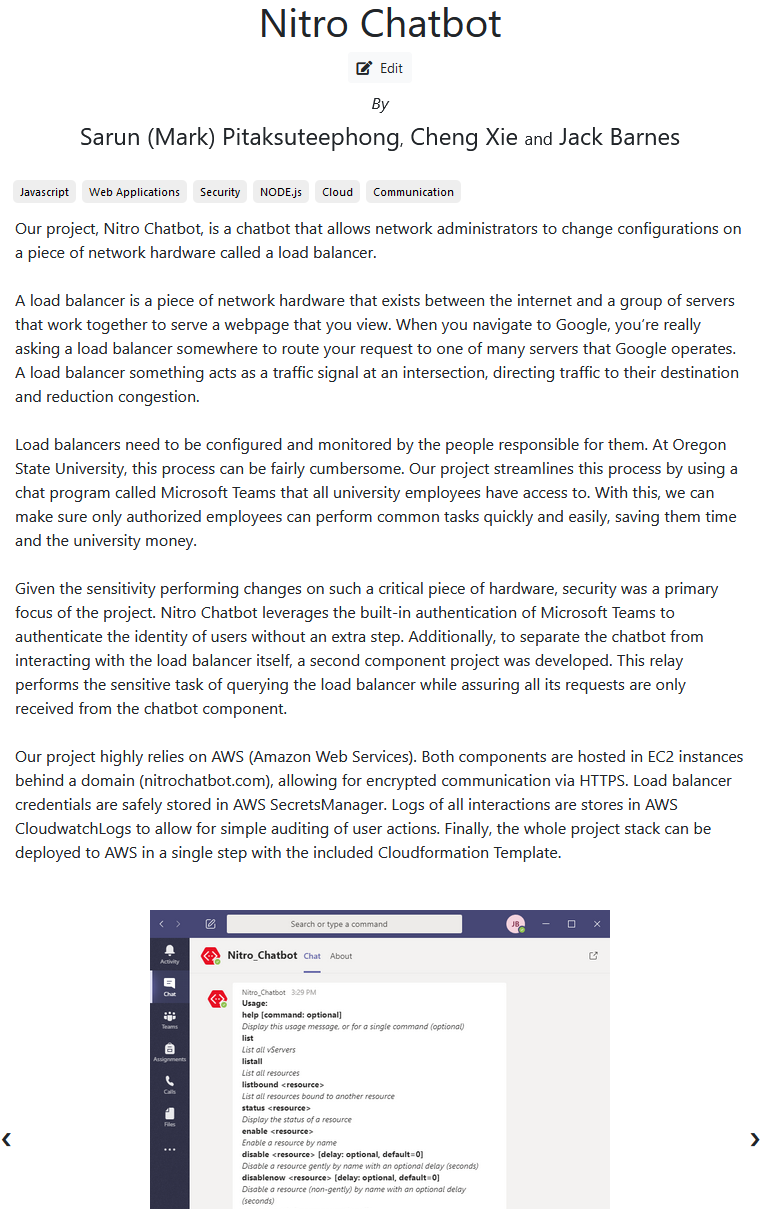
\includegraphics[height=20cm]{showcase.png}
        \label{fig:Final Showcase Image}
    \end{figure}

\section{Project Documentation}
\subsection{Overview}
This project is a chatbot for Microsoft Teams that allows authorized users to quickly query a NetScaler load balancer to view the status and enable/disable various resources.
Contained within are 2 Node.js projects that are meant to be deployed separately and interact with each other. Additionally there are 2 more folders, one for documentation and one for file pertaining to deployment.

\subsection{Repository Contents}
\subsubsection{Chatbot}
The first project is the chatbot (contained within /chatbot).
The chatbot uses BotKit to interact with Microsoft's Bot Framework.
For the chatbot to operate, it must be deployed and accessed with an https address (For deployment, we use a purchased domain: nitrochatbot.com).
Additionally, the chatbot must be registered as a Microsoft application to obtain a valid ID and Secret Key to be accessible through Microsoft Teams.
Finally, accessing the application requires an application manifest file (within the /deployment folder).

\subsubsection{Relay}
The second project is the relay (contained within /relay).
The relay acts as a web server (running with Express), accepting messages only from the chatbot.
Messages it receives are parsed and formulated into requests to the NetScaler (via it's REST API, NITRO).
The relay then passes responses to the chatbot so it can reply to the user.

\subsubsection{Deployment}
This folder contains relevant files pertaining to deployment of this project.
Additionally, this folder will contain the application manifest file that can be used to install NitroChatbot as an application within Microsoft Teams.

\subsection{Deploying the Project}
To deploy this project within AWS, a Cloudformation template deployment/NitroChatbot.json accurately describes all the resources needed to deploy both instances to AWS.

\subsubsection{Prerequisites}
\begin{enumerate}
    \item Existing Key-Pair within AWS to assign to both instances (the template will prompt for this)
    \item The bot needs to be registered with Microsoft's Bot Framework here
    \item You'll need both the App ID and an access key (which needs to be generated separately) when creating the stack from the template.
    \item URL for the Relay (this is given to the chatbot instance so that is can communicate with the relay using https).
    \item Full ARN for a pre-generated SSL certificate. This is used by both application load balancers.
    \item A TOTP Key. This is Base32 (A-Z,2-7) and must be 32 characters long. You can run the file totpgenks.js with node to generate a valid key.
\end{enumerate}

\subsubsection{Creating the Stack}
Use Cloudformation with the NitroChatbot.json for the template. Enter all the information gathered during the prerequites into the parameters. On average it took about 5-7 minutes to finish creating the stack.

Once the stack is created you'll be able to see both public DNS addresses within the Outputs. After the instances have finished initializing, you'll be able to verify their operation by visiting those addresses (make sure you prefix them with https://).

Note: You'll have to click through a certificate warning, since your browser will be recieving a certificate that doesn't match the address you browsed to.

The chatbot instance will give you a plain page that states which version of Botkit it's running. And the Relay instance will give you an error about missing fields in your request. This is a good sign.

The next step is to use the outputs you were given as ALIAS A Records for your hosted zone in Route 53.

Finally, from Microsoft Teams, install the application using the NitroChatbot.zip file.

Note: the manifest file contained within will need to be updated to match the URL of the Chatbot and it's application id.

\subsubsection{Adding Users}
To add an allowed user for Nitro Chatbot you'll need to create a new secret in SecretsManager.

The secret name needs to match their unique ID (users who use the command "request-auth" with the chatbot will have this value logged in the "RequestedAuths" log stream). The contents of the secret must be:
\begin{table}
    \caption{SecretsManager Entry}
    \centering
\begin{tabular}{| p{2.5cm} | p{5.0cm} |}
    \hline \textbf{Secret Key} & \textbf{Secret Value} \\
    \hline
    url & https://nitrourl.com/
    \\ \hline
    username & $<$their\_username$>$
    \\ \hline
    password & $<$their\_password$>$
    \\ \hline
\end{tabular}
\end{table}

\subsubsection{Final Notes}
I attempted to create a Macro to generate a TotpKey on stack creation, but could not get it to work (wasn't able to reference it from another template).
However, I did include the work I did in the file NitroChatbotGenKey.json.
This should be fixable with a little work.

One alternative to including a macro, would be to have the Lambda function run separately and store the key for the instances to read separately. This could be used to periodically re-roll the key for additional security. Unfortunately, we weren't able to implement this within our limited timeframe.

\subsection{Local Deployment}
Deploying this project so that it runs locally takes a large amount of system configuration to get setup correctly.

\subsubsection{Prerequisites}
These instruction are intended for use on Linux.
This project is untested on Windows, but could easily be adapted to that environment.
Additional, these instructions require the use of an AWS account.
Some of these procedures may result in charges.

The following software needs to be installed locally to run the project: Nodejs v14 and Bot Framework Emulator.

Clone the repository to a local folder.
Within the repository, add the following files: chatbot/.env chatbot/.app\_creds andrelay/.env

On the system add: ~/.aws/credentials

\paragraph{chatbot/.env}
2 lines are required in this file:
\begin{verbatim}
    RELAY_URL=
    TOTP_KEY=
\end{verbatim}

RELAY\_URL must be equal to the address for the relay when it's running.
In the case of running locally, this will be equal to http://127.0.0.1:3001 TOTP\_KEY must be a base32 key, probably of length 16 (other lengths will work however).
Base32 is uppercase letters A-Z and digits 2-7. This value must be matched within /relay/.env

\paragraph{chatbot/.app\_creds}
In .app\_creds there must be 2 lines, the first line is the Microsoft App ID, and the second line is the Microsoft App Password.
In the case of running locally, these lines may be empty, but they must be there (the bot does not need to authenticate with Microsoft correctly to run locally).

\paragraph{relay/.env}
This file needs 2 lines:
\begin{verbatim}
    PORT=
    TOTP_KEY=
\end{verbatim}

TOTP\_KEY must be set to the same value as it set in /chatbot/.env (base32) PORT is optional (defaulting to 3001 when not present), but I recommend still including this line so that we are explicit.

\paragraph{~/.aws/credentials}
Create this folder if it's not present and within the file create this structure, filling it in with the details for an AWS user:
\begin{verbatim}
    [default]
    aws_access_key_id = 
    aws_secret_access_key =
\end{verbatim}

The AWS user above must have a policy with these fields attached:
\begin{verbatim}
    {
    "Version": "2012-10-17",
    "Statement": [
        {
            "Effect": "Allow",
            "Action": [
                "secretsmanager:GetResourcePolicy",
                "secretsmanager:GetSecretValue",
                "secretsmanager:DescribeSecret",
                "secretsmanager:ListSecretVersionIds"
            ],
            "Resource": [
                "*"
            ]
        },
	      {
            "Effect": "Allow",
            "Action": [
                "logs:CreateLogGroup",
                "logs:CreateLogStream",
                "logs:PutLogEvents",
                "logs:DescribeLogStreams"
            ],
            "Resource": [
                "arn:aws:logs:*:*:*"
            ]
        }
    ]
}
\end{verbatim}

\paragraph{Create Log Group/Stream}
Next we must create an AWS CloudWatch Log Group and 2 Streams: In CloudWatch, go to Logs->Log groups.
Click Create log group and set it's name to NitroChatbot Inside the new log group, create 2 log streams: UserLogs and RequestedAuths

\paragraph{SecretsManager Authentication}
Next go to SecretsManager within AWS, and create a new custom Secret with the following fields:
\begin{verbatim}
    {
        "url": "https://netscaleraddress.com",
        "username": "nsroot",
        "password": "nsroot"
    }
\end{verbatim}

Set url to the address of your netscaler hardware/instance from the relay.
In the case of running locally or from AWS, this will be some public address username and password should be set to your credentials to access the NetScaler, nsroot/nsroot are default netscaler credentials.

The name of the secret will be your Microsoft global ID in this format (all lowercase hexadecimal): 
\begin{verbatim}
    xxxxxxxx-xxxx-xxxx-xxxx-xxxxxxxxxxxx
\end{verbatim}

You may choose to run a remote instance of Citrix ADC (this is a free AMI to use) within AWS to perform these operations against.
In this case, the default username is nsroot, and the default password is the instance id (viewable within the EC2 console).
Or you may run a version of the NetScaler software locally in a VM.
In this case, the default credentials are nsroot/nsroot.

\subsection{Running the Projects}
From the /chatbot directory, run "npm install" to install project dependencies, and then "npm start" to start the project.

In a different terminal, from the /relay directory, again run "npm install" to install the separate dependencies, and then npm start to run the project.

Now open Bot Framework Emulator, and select "Open Bot" and point it to the running chatbot application: 127.0.0.1:3000/api/messages.
Additionally, you may want to change your user id to match the name of your secret in SecretsManager.
This is something that can be done when running locally, but not in a production environment.

\subsection{Running the Tests}
Within each of the 2 projects is the ability to run test suites.
For our development pipeline, we have a separate Jenkins instance provisioned within AWS that automatically runs all our tests for each branch on each commit.
Viewing the commit history will show small icons next to the commit signifying if the commit passes all tests.
To run these tests locally you just need to navigate to the project folder and run the command "npm test".
The result of the tests will be output to the command line.

\section{Recommended Technical Resources for Learning More}
    The Chatbot portion of this project runs with BotKit framework.
    Their documentation can be viewed here: https://botkit.ai/docs/v4/
    
    The Relay uses express in order to run as a webserver.
    Their website includes a guide to it, as well as a full reference here: https://expressjs.com/
    
    When working with the NetScaler through the NITRO API, their documentation is invaluable: https://developer-docs.citrix.com/projects/citrix-adc-nitro-api-reference/en/latest/
    
    For building the Cloudformation template used for deployment, their user guide can be very helpful, providing a full reference: https://docs.aws.amazon.com/AWSCloudFormation/latest/UserGuide/Welcome.html
    
    Unit tests for this project were written using Jasmine, for more information about it see: https://jasmine.github.io/


\section{Conclusions and Reflections}
\subsection{Jack Barnes}
    First of all, I'm really proud of how the project turned out.
    The project not only works well, but I find that the code is very readable and should be very maintainable.
    A primary focus for our team was to not only make it work, but so that someone else could pick this up and continue to expand functionality.
    I really like the security implementation with the TOTP keys as well.
    
    I really learned so much, not just about writing code in JavaScript, but about AWS and DevOps in general.
    It was a huge challenge to develop something like this, that has so many connecting pieces.
    I cannot count the number of hours that I found myself digging through documentation to get everything working just right.
    
    I'm a bit amazed at the amount of different technology, systems, and software I got to work with throughout this project.
    In AWS alone I worked with EC2, CloudWatch Logs, SecretsManager, Cloudformation, Lambda, Route53, Certificate Manager, IAM, I tried building custom AMIs (which don't support BSD by the way), CLI, AWS-SDK, and probably more.
    I registered and deployed a domain behind HTTPS with multiple endpoints (Jenkins, NetScaler, Chatbot, and Relay).
    I used a remotely hosted Jenkins instance to receive web-hooks from GitHub, pull the code and run the tests, and then report the results back to GitHub.
    I worked with Citrix ADC software, particularly the load balancer, through the web interface and via it's REST API, NITRO.
    I registered our application with Microsoft's Azure Bot Service, which is required for Bots that run through their ecosystem of applications.
    I really feel that I'll be able to use all this knowledge going forward.
    
    The software engineering portion of the Capstone project was also a challenge.
    Project management and working together with peers in a team can be difficult, especially what you don't know what everyone will be bringing to the table.
    I've learned to be flexible, to maintain a high level of communication, and to be an organized as possible.
    I felt that communication with my group and with our client was vital to the groups success.
    
    If I has to do it all over again, knowing what I know now, I would definitely be able to come up with a slick UI for interacting with our bot.
    This is something I really didn't even know was an option until I was to see our application running within Teams.
    Much of my time was spent in learning and research. 
    More time for development would've only made the end result better.
    
    After completing this project, I can say for certain that it's helped me to become a better developer.
    I look forward to any and all challenges that I encounter next in my career.

\subsection{Cheng Xie}
    Overall, the senior capstone class is a very good class because it can let students know what is a project looks like and how to complete the project. In class, we are also need to work with our teammates to communicate and cultivate the team work which is also nice. This can help us to feel the real feeling in the future when we go to the company and work with colleagues.
    
    In our project Nitro Chatbot, my role in this project it to design a good and convenient user interface which user can use all features easily. The technical information I learned is that in an attempt to future-proof the chatbot, how to write using the Botkit Framework in Node.js. I also learned that how to use Node.js and allow the chatbot to provide quick access to the status and configuration options for the server pools that the users manage.
    
    I would say how to create a good format report is the non-technical information I learned in this class. In previous I always think that the format is not important and not using some technical writing format. But after done with the project, I understand the importance of using a good format in the document will let other people include yourself to read and understand the idea easily. Also the words I choose in the report is different than in other writing assignments.
    
    In our project work, there is many things I have learned. The most important one is teamwork. In previous, I always work alone like writing code assignments and think the team work is not important. But after finished this class, I changed my mind and think the team work is the most important factor in an engineering project. 
    
    I think our project management is really good because our individual part actually has connected each other. We need finish our own part on time and then we can connect them together. That helps me know how important is the time management. 
    
    Like I said, I learned how to communicate with teammates in our team and learn how to work with them together. I need finish my part early so other members can use my part to connect with their parts. Most important one is that when a problem need to be solved, I should not use aggressive works to chat with the teammates. We should sit down and discuss what should we do next. Then make a conclusion of that idea rather than always think myself.
    
    I would say if I do it all over, I would probably add some features like voice control to control our chat-bot and optimized some features like the method to connect to the server. Overall we meet all the requirements which is good enough!

\subsection{Sarun Pitaksuteephong}
    When we took the Software Engineering classes, we learn about the basics of how project development works and had a glimpse of what it is like through mini-projects.
    Now in the Capstone classes, we are doing real projects with real clients in a guided environment.
    Unlike the prerequisite Software Engineering classes, not only do we have to complete a project from scratch but we also have to make sure it can be handed over to the client smoothly as well.
    
    Before the start of this project, I have barely coded in JavaScript before so learning a new language is always nice.
    While I have known about the development cycle for a while now, I have never really focused on the deployment part of it.
    It really surprises me on how many tools and layers there is to this part of the cycle.
    For example, we use Amazon Web Services (AWS) as our foundation for this project and through it, it works with Cloudformation, EC2, Amazon Lambda, Docker, and many other tools. 
    Continuous integration, a concept we covered only in concept before this, is explored in finer details such as how to integrate it to a project and how to deploy it.
    
    Working as a team is usually a challenge for me and this time is no different, as communication and flexibility is key to the success of a team.
    I think the team did well when it comes to this as everyone is very accommodating for the project.
    I am not the best when it comes to communicating but I have tried to keep up on that wherever I can.
    We maintained a good relationship with our client and the team overall, as we usually sit and talk on any challenges we faced along the way instead of arguing about it, which creates a good work environment.
    
    Overall the project went really well and is ready to be passed onto our client.
    The code has been formatted to look clean and the documentation is well documented.
    
    If we have to do it again, I would do more prior research and experimentation like online labs to get a better grip on what is needed for this project.
    As I am unfamiliar with a project's deployment, most of my time was spent doing research and reading than experimenting and development.
    Besides that, I think having the chatbot be more predictive in nature would help the user in giving either updates or suggestion they may want to expand their options.
    
    This class is certainly very different from any classes before and I imagine that this is just what a real-world project looks like under a scope.
    I still have much more to learn to master these skills I have gained from this project but it is certainly many steps in a good direction and I look forward to what the future will offer.

\section{Appendix}
\subsection{Appendix 1: Essential Code Listings}
As stated above, Nitro Chatbot is essentially 2 separate components that work together in tandem.
In this section, we will walk through some of essential fragments of code that allow the project to function.

\subsubsection{Chatbot}
The first component is the Chatbot itself.
The Chatbot primarily receives input from the user via Microsoft Teams.
It is responsible for parsing the user input, forwarding the request to the Relay, recieving the Relay's response, logging the interaction, and sending a formatted response to the user.

    \paragraph{Bot Event}
    When the chatbot is loaded and running, it processes events.
    These event handlers are triggered based on how they are defined.
    Within chatbot/features folder is where most of the code is written for this component.
    Each file within the base of that folder (not it's sub-folders) is read in by the main application (bot.js).
    
    These events are ordered, bot alphabetically by file, and internally in the order they are written.
    This is best exemplified by the single event in the file "bot\_unmatched\_commands.js"
    \begin{figure}[ht]
        \centering
        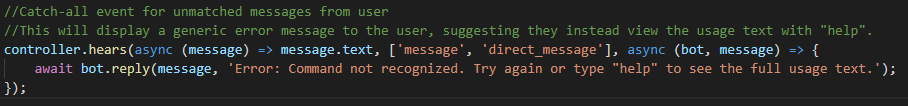
\includegraphics[height=2cm]{code1.png}
        \caption[Unmatched Bot Event]{This event will be triggered if the bot recieves a message, but it doesn't match any other defined event.}
        \label{fig:Unmatched Bot Event}
    \end{figure}
    
    This is the last event in the last file, triggering only when all other events aren't triggered first.
    
    For each basic command that the bot supports, an event is written with a regular expression that will match the event.
    This ordering principle is also used in ordering the commands, with the event for "list" coming after "listall" and "listbound".
    This allows a slightly more relaxed regular expression that will, in return, generate more precise error messages upon parsing the message.
    
    The first event in "bot\_relay\_commands.js" is for the listall commands:
    \begin{figure}[ht]
        \centering
        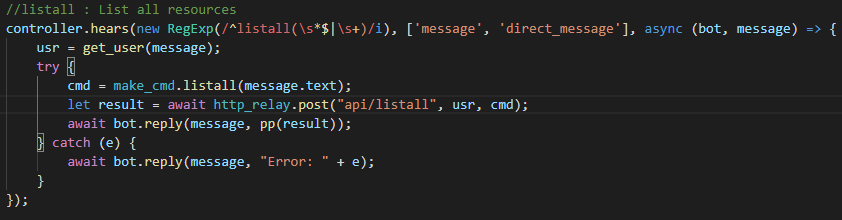
\includegraphics[height=3cm]{code2.png}
        \caption[Event For listall]{This event will be triggered when the message matches the Regex}
        \label{fig:Event For listall}
    \end{figure}

    Each event has similar formatting, performing the same sequence of actions.
    The first is get\_user(message), which pulls the unique id for the user from the message object.
    The next actions are wrapped in a try-catch block.
    This is because both make\_cmd and http\_relay are designed to throw an error with a descriptive string that can be sent directly to the user.

    \paragraph{Making the Command Object}
    Within make\_cmd (at chatbot/features/lib/cmd/make\_cmd.js), each command's requirements are defined by the functions it calls with it's input.
    The purpose of this library is to return an object that is standardized for the relay to understand, and free from bad inputs that the user may give.
    
    \begin{figure}[ht]
        \centering
        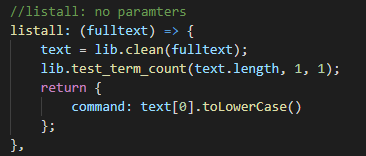
\includegraphics[height=2cm]{code3.png}
        \caption[Make\_Cmd for listall]{This library function produces the standardized command object that they relay expects}
        \label{fig:Make_Cmd For listall}
    \end{figure}

    Each of these library functions calls of set of functions contained within cmd\_lib.js.
    This allows each function to throw a descriptive error back to our triggered event, and pass the error to the user.
    Each function called from here has a set of tests to assure their proper operation.
    In this example function you can see that the only requirement is that the message have a single term (the command name itself).
    
    \paragraph{HTTP to Relay}
    The next function that the event will call is from chatbot/features/util/http\_relay.js.
    Here, axios, an external module, will create a POST request to the base url set from the environment variable RELAY\_URL.
    The request body takes this form:
    
    \begin{figure}[ht]
        \centering
        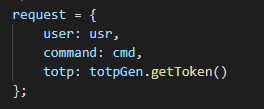
\includegraphics[height=2cm]{code4.png}
        \caption[Request Body to Relay]{This request object is used as the request body to the Relay from the Chatbot}
        \label{fig:Request Body to Relay}
    \end{figure}

    Here the user sub-object contains the requesting user's information.
    The command sub-object contains the relevant information about the request.
    
    TOTP is a 6 digit number that's generated by a symmetric key which both the Chatbot and Relay are given during deployment.
    This TOTP key is generated from using the RFC 6238 standard, and relies on code written for the totp-generator 0.0.7 (available here: https://github.com/bellstrand/totp-generator).
    Our use of the code wraps the library in an object that pre-stores the symmetric key so we don't need to pass it in every time we generate a new key.
    
    TOTP works by using a secret key and the current time to generate a different key every 30 seconds.
    This allows the Relay to authenticate requests from the Chatbot, while making guessing the correct key within the time-limit very difficult for any potential attacker.
    An idea for an improvement to this scheme is available in Appendix 2.
    
    \begin{figure}[ht]
        \centering
        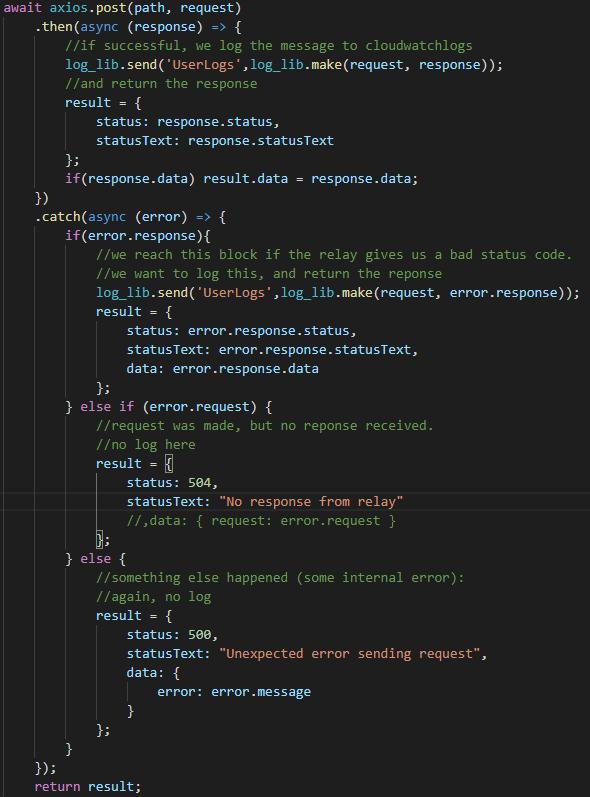
\includegraphics[height=12cm]{code5.png}
        \caption[Sending Request to the Relay]{This call using axios handles the logic for how responses are processed.}
        \label{fig:Sending Request to the Relay}
    \end{figure}
    
    When sending the request to the relay there are 4 possible results.
    The first result is that the call is successful (meaning the relay responded with the request with some 2xx status code).
    In this case the result is logged, and the result is returned to the chatbot.
    
    The second case is an error response sent back from the relay.
    This interaction is also logged, and the result is returned to the chatbot.
    
    The third and forth cases are either the Relay didn't respond, or that there was some unexpected error sending the request.
    In these cases, the result is not logged, but is still returned to the chatbot.
    
    \paragraph{Responding to the User}
    After the result is received from http\_relay,  bot.reply is called to reply to the user who sent the command.
    This is a function provided by the chatbot framework, BotKit.
    The second parameter is the message we wish to reply with.
    The format it for the user, we use chatbot/features/util/pretty\_print\_json.js.
    
    \begin{figure}[ht]
        \centering
        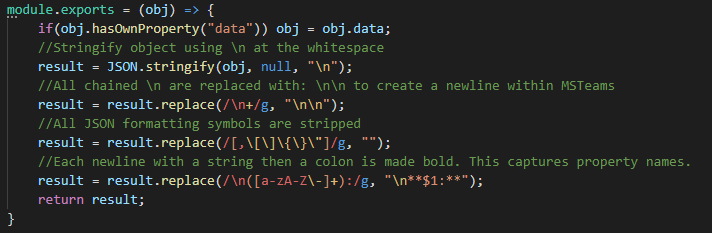
\includegraphics[height=3.5cm]{code6.png}
        \caption[Processing the Relay's Response]{This pretty-print function processes the output and to string that formats nicely in Microsoft Teams}
        \label{fig:Processing the Relay's Response}
    \end{figure}
    
    Here we use some regex to strip out some characters and apply some simple formatting.
    Processing the text in this way lets the Relay send any information back that it wants, allowing the developer to add or remove fields from the response without worrying about frontend processing.
    It is trivial to add or remove fields from each status command (the result being different for each resource-type).

\subsubsection{Relay}
    The second project component is the Relay.
    The Relay is responsible for authenticating the user, sending a request to the NetScaler, and responding to the Chatbot.
    
    \paragraph{Middleware}
    The relay runs as an express server, utilizing custom middleware to process every request.
    Each different command sent by the user triggers a different route, but utilizing middleware allows for common processing to be abstracted from the route itself.
    
    \begin{figure}[ht]
        \centering
        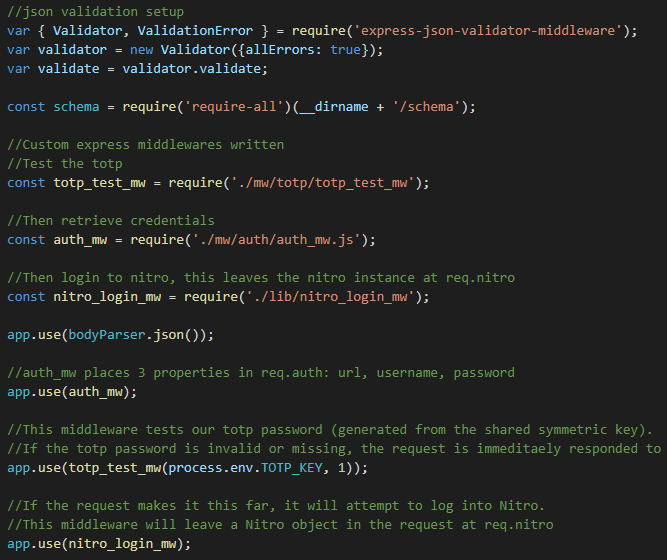
\includegraphics[height=8cm]{code7.png}
        \caption[Middleware for Relay]{This is all the middleware that is utilized by the relay}
        \label{fig:Middleware for Relay}
    \end{figure}
    
    First, auth\_mw attempts to authenticate the user ID against our list of authenticated users in AWS Secrets Manager.
    Next the TOTP key is tested, if the key is valid then the request is processed further.
    Otherwise nothing else will happen (see Appendix 2 for improvements to this ordering).
    
    The last line of this figure using the credentials gathered in auth\_mw to authenticate with the Netscaler, storing a session token in a new instance of our nitro library.
    This methodology saves the authenticated instance of the library as a sub-object of the request.
    This lets the written routes for the Relay to avoid handling the token directly.
    
    \paragraph{Routes}
    \begin{figure}[ht]
        \centering
        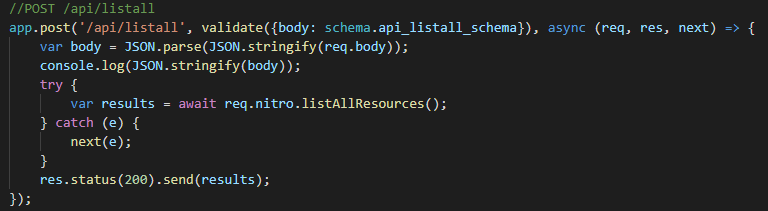
\includegraphics[height=3cm]{code8.png}
        \caption[Relay's Route Logic]{This is the logic for the api/listall route on the Relay}
        \label{fig:Relay's Route Logic}
    \end{figure}
    Each route implementation has been made very simple in an effort to improve readability.
    Before any body of the route is run however, validate verifies the body has the correct structure.
    This is through the use of the JSON Schema files (contained at relay/schema/).
    The schema files allow for the request body to be verified and assured that they contain valid values.
    In order to support more commands, another schema file will need to be created to match the needs of the command.
    
    Each use of the nitro library functions is always wrapped in a try-catch block.
    This is because the nitro library will always throw errors when it encounters problems, such as requesting the NetScaler for resources that don't exist.
    In the catch block, next(e) is called.
    This is functionality within express that lets us pass an error to an error handling function.
    
    \paragraph{Handling Errors with Express}
    \begin{figure}[ht]
        \centering
        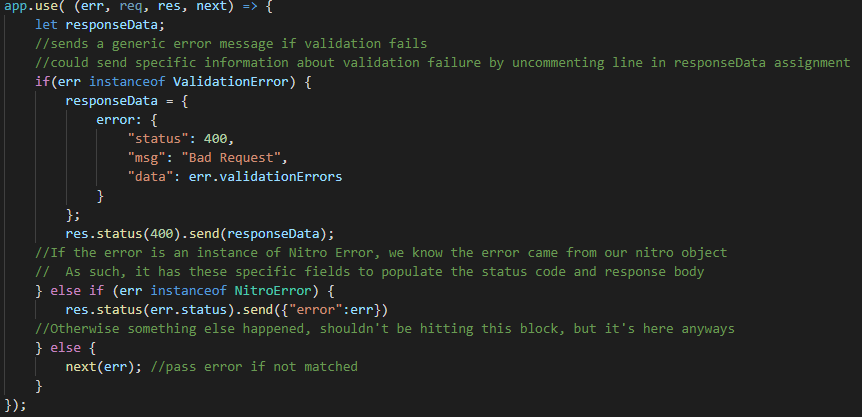
\includegraphics[height=6cm]{code9.png}
        \caption[Handling Errors]{This is the special route that we can call by passing a value to next()}
        \label{fig:Handling Errors}
    \end{figure}
    
    This function has been design to capture 2 types of errors.
    The first error is a Validation Error, this is generated by the schema validation middleware library that we are using.
    The second error is a NitroError, which is a standardized error object that we've written to represent all errors.
    When encountering an error, the Nitro library will generate an object of this time and throw it.
    We then catch it with out use of try-catch blocks.
    This allows all error to produce custom error messages and status codes to most accurate represent the error that occurred.
    
    \paragraph{Nitro Library}
    All of this code is contained within the directory relay/lib/nitro.
    The base file, nitro.js provides the access interface for the relay to use.
    All logic required to complete each of these commands has been pushed to this level, or into one of the child files (nitro\_util.js, nitro\_list.js, and nitro\_list\_all.js).
    
    \begin{figure}[ht]
        \centering
        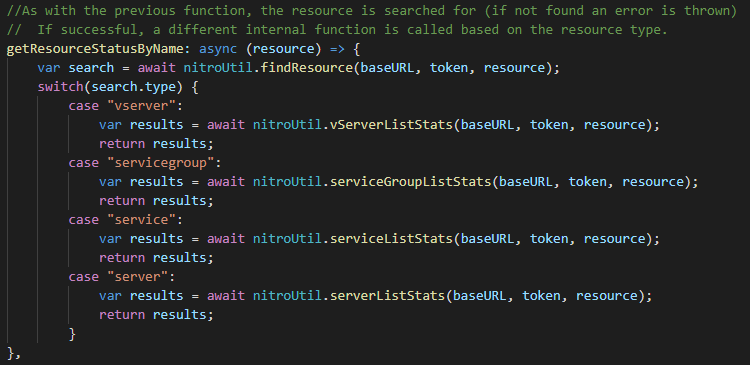
\includegraphics[height=6cm]{code10.png}
        \caption[Get Resource Status]{This function is called when issuing the status command. It generates multiple calls to the NetScaler}
        \label{fig:Get Resource Status}
    \end{figure}
    
    In this internal function, getResourceStatusByName, first the library must attempt to find the resource only by name.
    This works because each resource name on the NetScaler must have a unique name.
    Knowing this, we can use the findResource function, which generates 4 different calls, enumerating all the names of each of the 4 types of resources we are dealing with (vserver, servicegroup, service, and server).
    Using that we can call the appropriate function.
    
    \begin{figure}[ht]
        \centering
        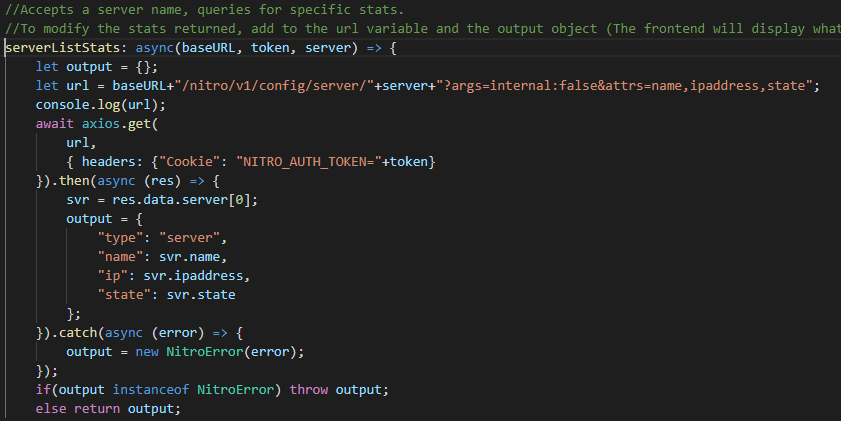
\includegraphics[height=6cm]{code11.png}
        \caption[Nitro Library Function]{serverListStats makes the actual call to the NetScaler, using it's REST API, NITRO}
        \label{fig:Nitro Library Function}
    \end{figure}
    
    If you were to query the status of a server resource, eventually this function will be called.
    The actual fields that we return to the user are set here.
    First we set the fields as query parameters in the url, and then again in the output object we return.
    We can also set friendly names here, as this is what the user will eventually see.
    
    In the event of an error, we create a NitroError object from a class using new.
    This is what lets us use instanceof to check for errors, instead throwing the output to be caught by the error route.
    This methodology was used to avoid passing around error flags or check for incomplete responses at a highly level.
    
    From here, results are passed all the way back to the user to see from within Microsoft Teams.

\subsection{Appendix 2: Further Work}
\subsubsection{Remaining Bugs}
    Unfortunately some small bugs still exist with the system as it stands today.
    
    The first bug is that the chatbot doesn't properly respond when enabling or disabling resources.
    This is likely to be a very small bug and would have been fixed if it were noticed before the team's deadline.
    This bug had previously occurred and was fixed with some simple logic updating in the pretty-print function that is used by the Chatbot.
    
    The second bug is a bit larger.
    Within the current implementation, the timed delay for disable doesn't appear to be working as expected.
    While the nitro library appears to be using the disable route correctly, an error may still persist.
    However, this may also not be a bug, and could actually be expected behavior of the NetScaler (as we only used one without traffic).
    Careful examination of this functionality is recommended to any future developer.

\subsubsection{Adding a New Command}
    A major focus of the final project refactoring, was to make it expandable with more commands.
    Here I'll list each file and describe the revision.
    For the most part, following the flow through an existing command should help anyone unfamiliar with the project's code.
    
    \paragraph{Chatbot}
    First bot\_relay\_commands.js will need to have an event created for the next command.
    Substitute in the name of the new command in the regular expression for the event, for the called function within make\_cmd and the destination url in the first parameter of the http\_relay.post() call.
    
    Next make\_cmd.js needs to have a function added for your new command.
    You can copy and existing one and modify based on the requirements you wish to set for the command.
    
    Next go to usage.js and add in your next command into the usage object following the template of the existing commands.
    
    Now go to cmd\_lib.js, in here you'll need to add your new command to the list of available commands in test\_command\_param(). This will let the user request the help text for your new command directly.
    
    \paragraph{Relay}
    In the main project file, relay.js create a new route by copying an existing one, and changing the target to the same url you set in the chatbot.
    Change the target schema name to the new schema you'll be creating.
    Also update the nitro function call to the name of the new function you'll be creating.
    
    To make a new schema file, copy and existing one and make any required changes to match the data you need to send from the chatbot (which you've already set in the make\_cmd function).
    
    Now navigate to nitro.js and create the new function you've already named in relay.js.
    From here you'll have to program the needed logic for your new custom command based on the existing functions (start by copying one and modifying to suit your use-case).
    It's highly recommended to have the NITRO API documentation open for reference, and potentially some tool like Postman to test requests before coding them.

\subsubsection{Improving Security/TOTP}
    The first suggestion for improving security would be to place the TOTP middleware within the relay project first, so that it is the first test that is run. This could be a security issue when run in production.
    
    The next suggestion would be to increase the size of the TOTP key that is used.
    A six digit code is very small in terms of security, even with it refreshing every 30 seconds.
    A determined third party with enough information of the system is likely to find a way to defeat this security given time.
    There is likely better methodology to assure that only the Chatbot communicates with the Relay.
    
    That said, the TOTP system is a nice solution to the problem that the team encountered.
    One way to improve it would be to expand the size of the key.
    This could be done with a small modification to the totp\_gen\_mod.js file.
    This tactic would be worth investigation.

\subsection{Appendix 3: Code Review Critiques and Responses}
\subsubsection{Fixed Bugs}
During the live demo of the code review, I spotted 2 small production errors that have been resolved.
\begin{enumerate}
    \item Angle brackets not showing on the usage message command: help
    \item The Teams Linux client was unable to pass the schema tests on the relay.
\end{enumerate}

\subsubsection{Feedback Forms}
As a team, we received a total of 3 feedback forms.
The feedback was overwhelmingly positive, and contained very little correction or potential improvements.
Here I will discuss the feedback we received so as to assure the grader that we've carefully considered the feedback.
\paragraph{More Comments?}
One suggestion that we received was to further comment the code, especially parts dealing with authentication and other external requests.
As a result of this feedback we've added (or modified) 84 lines of comments to our code.
\paragraph{Fuzz Testing?}
The other only suggestion we received was for fuzz testing.
This was suggested by 2 people, to presumably, test routes and other forms of input.
As we discussed during our code review, we didn't think it was feasible to implement this in a way that would provide meaningful information at this point.
But, allow me to explain the project and our thought process here (apologies if the explanation is a bit long-winded).

Essentially, in production, the chatbot will only receive input from Microsoft, as it handles the messages sent from users.
The chatbot itself is registered with Microsoft and uses an application ID and password given by Microsoft.
The chatbot component of the project is built with BotKit.
Tests down this path would either be testing Microsoft, or the framework, BotKit, itself (owned by Microsoft).
However, user input itself is thoroughly tested and carefully sanitized.

The second target of additional testing could be the Relay itself.
However, our system employs a shared symmetric key, and verifies the key with each request by use of a 6-digit TOTP password that rolls over every 30 seconds.
Every request that doesn't match a current key is discarded.

Additionally all requests that do reach the relay must exactly match the json schemas designed for each request. This includes careful regex matching.
UserIDs are then matched against a database, and credentials for only that user are retrieved and never stored within the relay.

With this system, we find that while additional testing may be possible (essentially customized end-to-end testing), it's simply not worth the time it would take for us to implement.

\subsubsection{Requirements Met}
All feedback we received during the code review agree that our project meets the requirements given in the updated version of the requirements document.

\subsubsection{Deployment}
Although not this is not a strict requirement set forth in the requirements document, we know that our client would like to see a Cloudformation template that accurately describes our AWS configuration.
To this end, the final submission to our repository before code freeze is within a new folder "deployment".
This contains a json file to be used to deployment the required resources and standup the instances required to use our project.

That's it for our code review response. Thanks!

\clearpage
\subsection{Appendix 4: Feature Implementation Timeline}
\begin{figure}[ht]
    \centering
    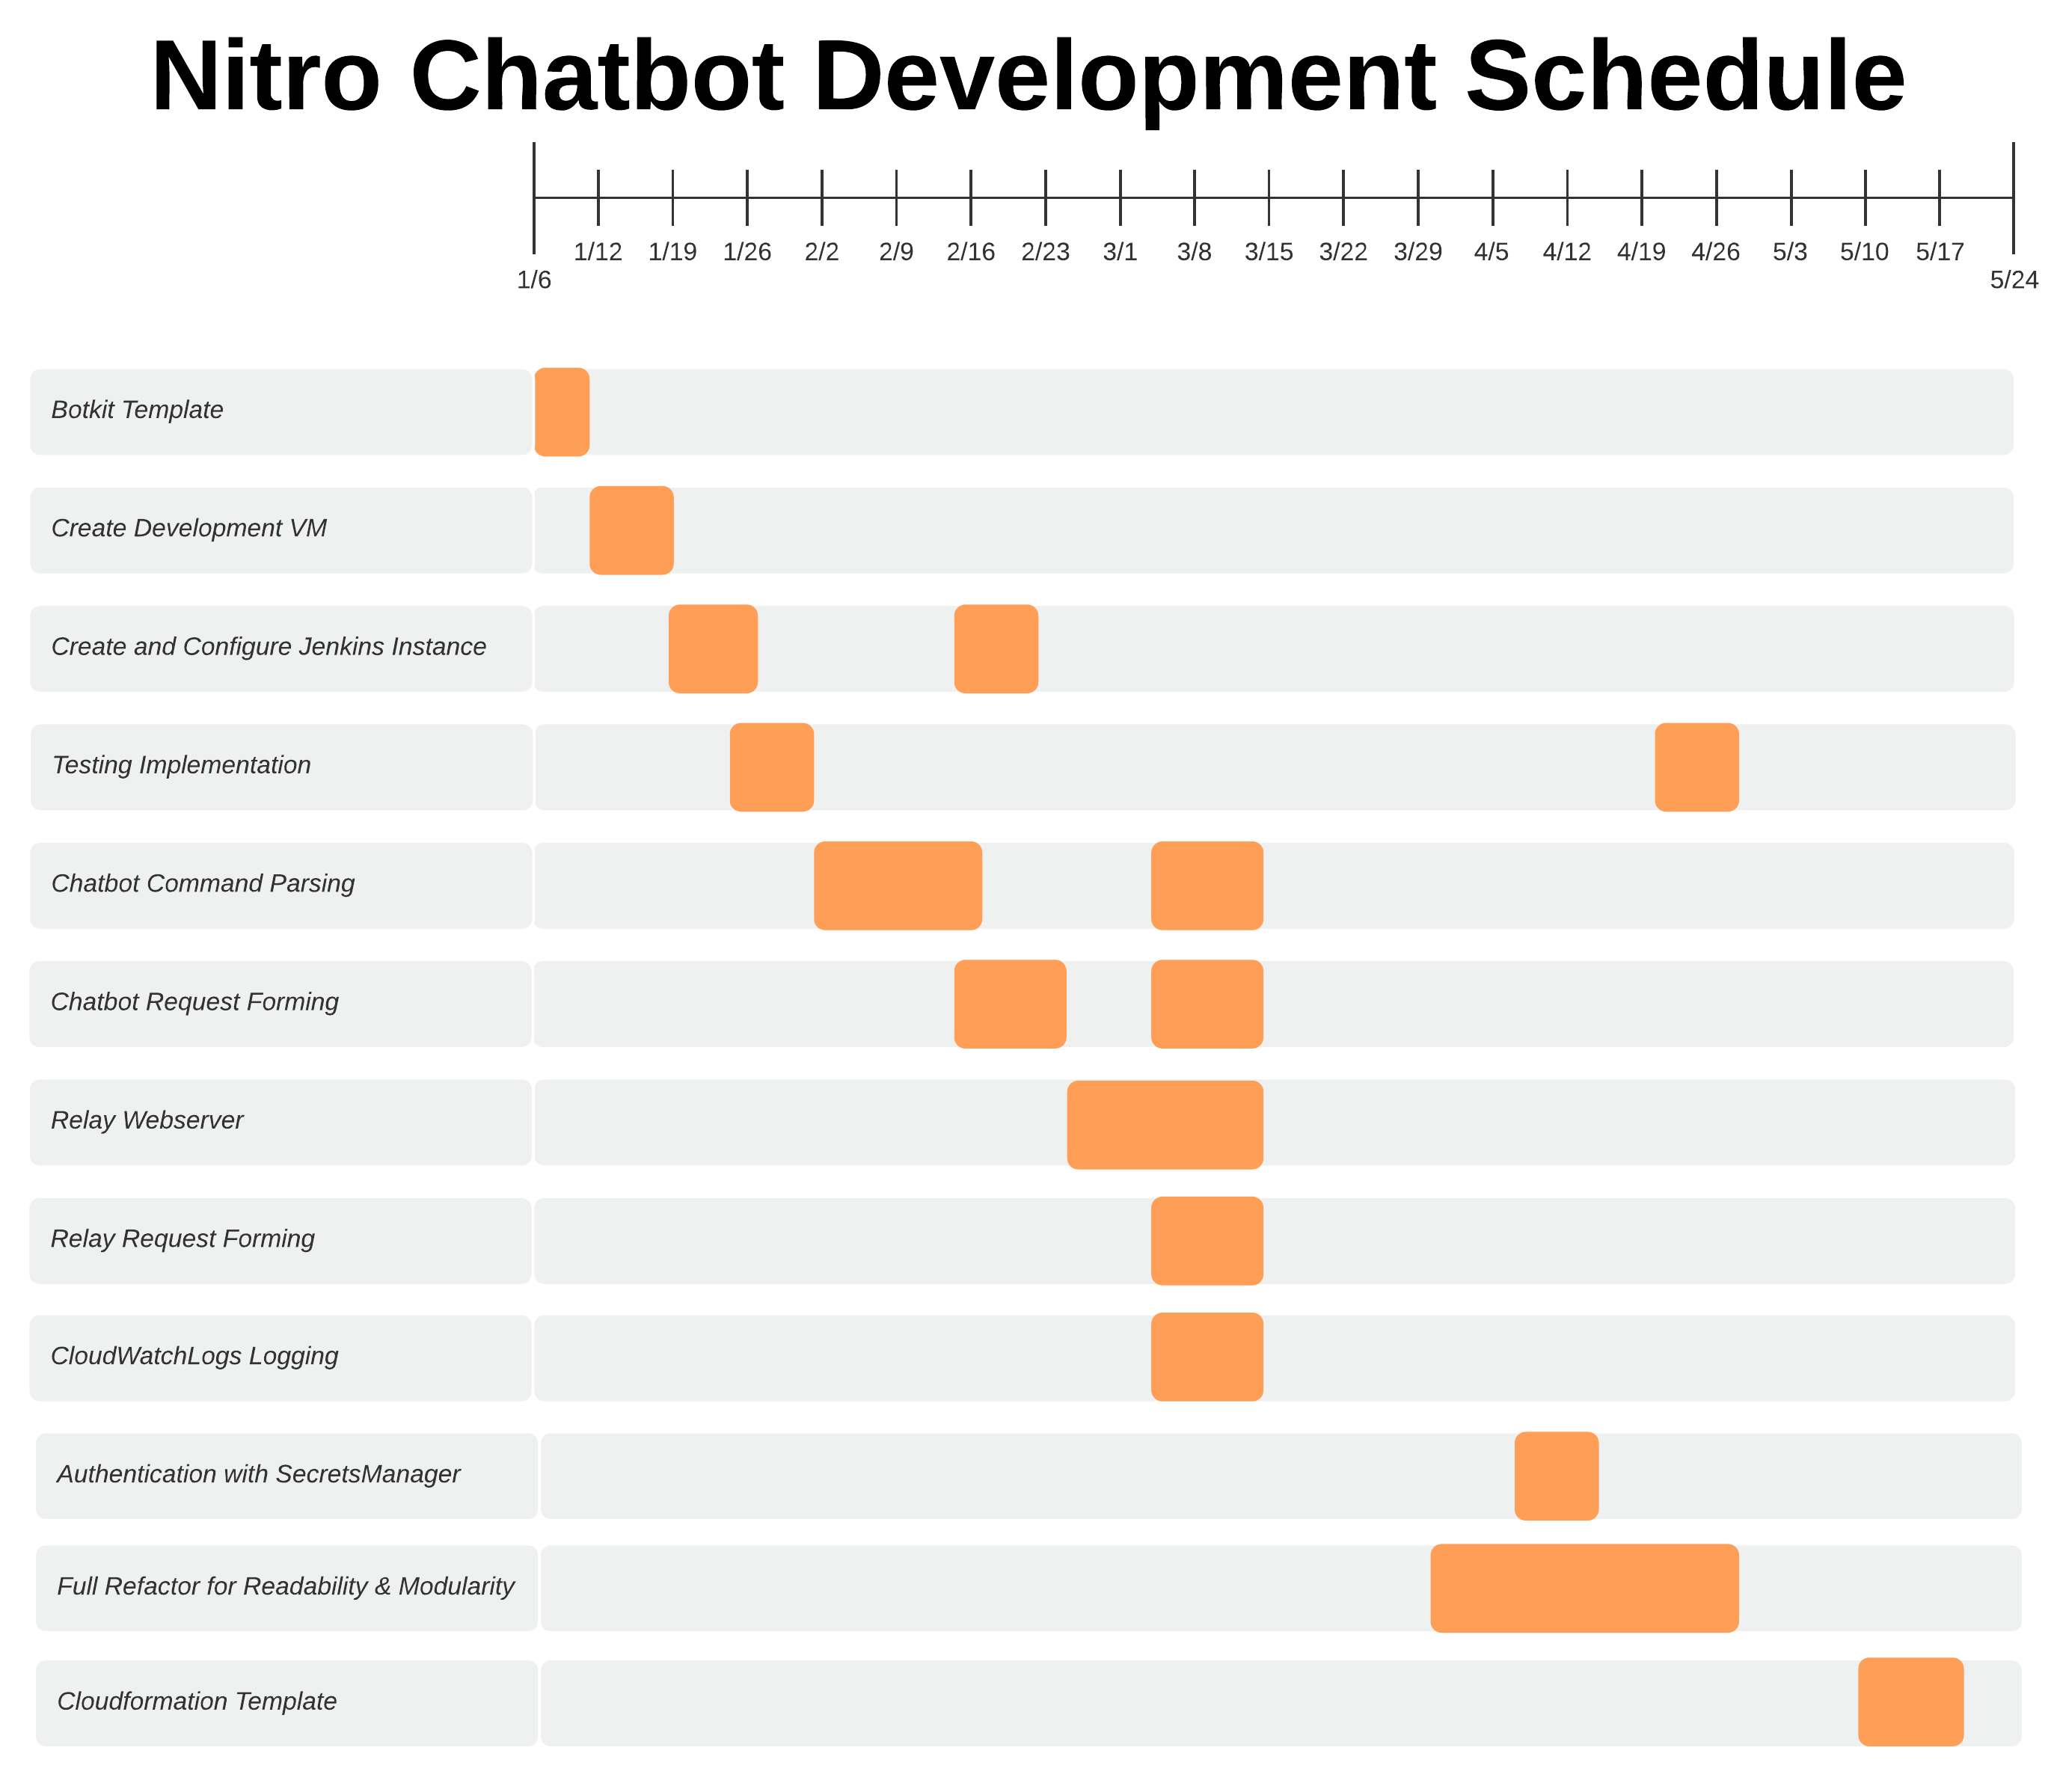
\includegraphics[height=15cm]{gantt-v2.png}
    \caption[Feature implementation timeline]{This is the actual development time for Nitro Chatbot.}
    \label{fig:Feature implementation Timeline}
\end{figure}

\clearpage
\bibliographystyle{IEEEtran}
\bibliography{all}

\end{document}
